\documentclass[degree=master]{thuthesis}
% 选项:
%   degree=[bachelor|master|doctor|postdoctor], % 必选
%   secret,                                     % 可选
%   pifootnote,                                 % 可选(建议打开)
%   openany|openright,                          % 可选,基本不用
%   arial,                                      % 可选,基本不用
%   arialtoc,                                   % 可选,基本不用
%   arialtitle                                  % 可选,基本不用

% 所有其它可能用到的包都统一放到这里了,可以根据自己的实际添加或者删除。
\usepackage{thuthesis}
\usepackage{algorithm}
\usepackage{algorithmic}
\renewcommand{\algorithmicrequire}{ \textbf{Input:}}      %Use Input in the format of Algorithm
\renewcommand{\algorithmicensure}{ \textbf{Output:}}     %UseOutput in the format of Algorithm

\usepackage{url}
\usepackage{listings}
\usepackage{xcolor}
\lstset{
    numbers=left,
    numberstyle= \tiny,
    keywordstyle= \color{ blue!70},
    commentstyle= \color{red!50!green!50!blue!50},
    frame=shadowbox, % 阴影效果
    rulesepcolor= \color{ red!20!green!20!blue!20} ,
    escapeinside=``, % 英文分号中可写入中文
    xleftmargin=2em,xrightmargin=2em, aboveskip=1em,
    framexleftmargin=2em
}

% 定义所有的图片文件在 figures 子目录下
\graphicspath{{figures/}}

% 可以在这里修改配置文件中的定义。导言区可以使用中文。
% \def\myname{薛瑞尼}

\begin{document}

%% 封面部分
\frontmatter
\thusetup{
  %******************************
  % 注意:
  %   1. 配置里面不要出现空行
  %   2. 不需要的配置信息可以删除
  %******************************
  %
  %=====
  % 秘级
  %=====
  secretlevel={公开},
  secretyear={2100},
  %
  %=========
  % 中文信息
  %=========
  ctitle={基于集中平台的RSCP-iBGP系统的研究与实现},
  %清华大学学位论文 \LaTeX\ 模板\\使用示例文档 v\version},
  cdegree={工学硕士},
  cdepartment={计算机科学与技术系},
  cmajor={计算机科学与技术},
  cauthor={王庆},
  csupervisor={尹霞教授},
  %cassosupervisor={陈文光教授}, % 副指导老师
  %ccosupervisor={某某某教授}, % 联合指导老师
  % 日期自动使用当前时间,若需指定按如下方式修改:
  % cdate={超新星纪元},
  %
  % 博士后专有部分
  cfirstdiscipline={计算机科学与技术},
  cseconddiscipline={系统结构},
  postdoctordate={2009年7月——2011年7月},
  id={编号}, % 可以留空: id={},
  udc={UDC}, % 可以留空
  catalognumber={分类号}, % 可以留空
  %
  %=========
  % 英文信息
  %=========
  etitle={A Study and Implement Based on Centralized Platform of RSCP-iBGP System},
  % 这块比较复杂,需要分情况讨论:
  % 1. 学术型硕士
  %    edegree:必须为Master of Arts或Master of Science(注意大小写)
  %             “哲学、文学、历史学、法学、教育学、艺术学门类,公共管理学科
  %              填写Master of Arts,其它填写Master of Science”
  %    emajor:“获得一级学科授权的学科填写一级学科名称,其它填写二级学科名称”
  % 2. 专业型硕士
  %    edegree:“填写专业学位英文名称全称”
  %    emajor:“工程硕士填写工程领域,其它专业学位不填写此项”
  % 3. 学术型博士
  %    edegree:Doctor of Philosophy(注意大小写)
  %    emajor:“获得一级学科授权的学科填写一级学科名称,其它填写二级学科名称”
  % 4. 专业型博士
  %    edegree:“填写专业学位英文名称全称”
  %    emajor:不填写此项
  edegree={Master of Science},
  emajor={Computer Science and Technology},
  eauthor={Wang Qing},
  esupervisor={Professor Yin Xia},
  %eassosupervisor={Chen Wenguang},
  % 日期自动生成,若需指定按如下方式修改:
  % edate={December, 2005}
  %
  % 关键词用“英文逗号”分割
   ckeywords={内部边界网关协议, 集中平台, 路由存储, 路由策略, 路由计算},
   ekeywords={Internal Border Gateway Protocol, Centralized Platform, Routing Storage, Routing Policy, Routing Calculation}
}


% 定义中英文摘要和关键字
\begin{cabstract}
  随着网络规模的不断扩大,自治系统内部需要逻辑全连接的内部边界网关协议iBGP,面临可扩展性问题。已有的研究方案路由反射、AS联邦、SoftRouter、RCP、RFCP等解决了iBGP的可扩展性,但带来了新的挑战。本文基于集中式体系结构的思路,提出基于集中平台的RSCP-iBGP系统,并充分利用集中平台的优势,在解决iBGP的可扩展问题的同时,也优化了路由存储和路由计算。如果自治系统内有N台边界路由器,iBGP全连接需要维护N平方的iBGP连接,路由表存储需要N份,在路由收敛的过程中路由计算需要最坏N平方次,而文中的新方案仅需维护N的iBGP连接,路由表存储O(1)份,路由表最坏计算N次。基于集中平台的RSCP-iBGP系统下,路由存储大小和路由计算次数均下降了一个数量级,该系统使得内部域间路由协议iBGP的性能、可扩展性提升很多。

  本文主要开展了以下工作:
  \begin{itemize}
    \item 针对iBGP可扩展问题,提出了基于集中平台的RSCP-iBGP系统,其中对路由存储、路由计算进行了优化,并将该系统与已有的5种方案进行对比分析,明确RSCP-iBGP系统相比于现有研究方案的优势。
    \item 设计RSCP-iBGP系统的工作流程、具体模块以及复式的最优路由计算算法,实现RSCP-iBGP系统中的三大模块:边界路由器,路由控制平台上的Route-Server,以及边界路由器与Route-Server之间的通信协议。
    \item 通过实验,对RSCP-iBGP系统进行功能验证。通过一致性测试工具PITSv3编写测试例对RSCP-iBGP系统进行功能一致性测试,最终验证了RSCP-iBGP系统的功能和设计相一致。
  \end{itemize}

\end{cabstract}

% 如果习惯关键字跟在摘要文字后面,可以用直接命令来设置,如下:
% \ckeywords{\TeX, \LaTeX, CJK, 模板, 论文}

\begin{eabstract}
   With the continuous expansion of network scale, internal border gateway protocol iBGP which requires a logical full mesh occurs scalability issue. Previous studies have solved the iBGP scalability issue, but brings new challenges, such as route reflection, AS federation, SoftRouter, RCP, RFCP, etc. This thesis proposes RSCP-iBGP system based on centralized platform to solve the iBGP scalability issue, which also optimizes routing storage and routing calculation. If there are N border routers in one Autonomous system, Full-Mesh IBGP needs to maintain N squared iBGP connections, to store N routing tables , and routing computing needs to execute N squared times in the process of routing convergence. RSCP-iBGP system only needs to maintain N iBGP connections, about one storage routing table, and routing computing needs to execute N times. The RSCP-iBGP system based on centralized platform contributes that size of routing storage and the number of routing computation are both reduced by an order of magnitude, And it improves the internal inter-domain routing protocols iBGP performance and scalability. The contributions of the work include:

   \begin{itemize}
    \item To solve scalability issue, the thesis puts forward the RSCP-iBGP system based on centralized platform, which optimizes routing storage and routing calculation. By comparing RSCP-iBGP system with and existing five schemes, the advantages of RSCP-iBGP system are confirmed.
    \item Design the work process, specific modules, multiple routing calculation algorithms, and RSCP-iBGP system realized three modules: border router, Route-Server running in the route control platform and the communication protocol.
    \item Execute functional verification of RSCP-iBGP system. The conformance testing of the RSCP-iBGP system was conducted by the conformance testing tool PITSv3, which finally verified that the realization of the RSCP-iBGP system is consistent with the design.
  \end{itemize}
\end{eabstract}




% \ekeywords{\TeX, \LaTeX, CJK, template, thesis}

% 如果使用授权说明扫描页,将可选参数中指定为扫描得到的 PDF 文件名,例如:
% \makecover[scan-auth.pdf]
\makecover

%% 目录
\tableofcontents

%% 符号对照表
\begin{denotation}[3cm]
\item[BGP] 边界网关协议(Border Gateway Protocol)
\item[iBGP] 内部边界网关协议 (Internal Border Gateway Protocol)
\item[eBGP] 外部边界网关协议 (External Border Gateway Protocol)
\item[EGP] 外部网关协议(Exterior Gateway Protocol)
\item[IGP] 内部网关协议(Interior Gateway Protocol)
\item[AS] 自治系统(Autonomous System)
\item[RR] 路由反射器(Router Reflector)
\item[RCP] 路由控制平台(Route Control Platform)
\item[RFCP] 路由流控制平台(Route Flow Control Platform)
\item[TCP] 传输控制协议(Transmission Control Protocol)
\item[MED] 多出口鉴别符(Multi-Exit Discriminators)
\item[SDN] 软件定义网络(Software-Defined Network)
\item[IXP] 网络交换节点(Internet Exchange Point)
\item[SDX] 软件定义的网络交换节点(Software Defined IXP)
\item[RSCP-iBGP] 基于路由控制平台的内部边界网关协议(Route Server Control Platform Internal Border Gateway Protocol)
\item[ASN] 自治系统号(Autonomous System Number)
\item[RIPv1] 路由信息协议版本1(Routing Information Protocol, Version 1)
\item[RIPv2] 路由信息协议版本2(Routing Information Protocol, Version 2)
\item[RIPng] 下一代路由信息协议(Routing Information Protocol, Next Generation)
\item[OSPFv2] 开放式最短路径优先版本2(Open Shortest Path First, Version 2)
\item[OSPFv3] 开放式最短路径优先版本3(Open Shortest Path First, Version 3)
\item[BGPv4+] 边界网关协议版本4扩展(Border Gateway Protocol, Version 4+)
\item[IS-IS] 中间系统到中间系统(Intermediate System-to-Intermediate System)
\item[PITSv3] 协议集成测试系统版本3(Protocol Integrated Test System, Version 3)
\end{denotation}



%%% 正文部分
\mainmatter
\chapter{引言}
\label{cha:intro}


\section{研究背景}

随着互联网的不断发展,自治系统的规模不断扩大,自治系统内的边界路由器数目和自治系统向外宣告前缀数目不断增加,互联网的域间路由协议面临多方面的挑战。边界网关协议(Border Gateway Protocol,BGP)是目前互联网使用的唯一的域间路由协议,直接影响网络功能和端到端的传输。早期设计BGP协议的阶段,自治系统(Autonomous System,AS)的数量和自治系统内部的边界路由器数量均较小,对BGP协议的可扩展性、安全性、路由策略的灵活性等缺乏关注。

BGP在AS内部所有路由器两两之间建立iBGP(Internal Border Gateway Protocol, iBGP)会话以交换域间路由,iBGP会话的数量是路由器平方数量级的,大型AS内部边界路由器的数目几百到上千,难以承受巨大的iBGP负担。学术界2000年左右提出了路由反射(Router Reflector, RR)和AS联邦的解决方案,两种方案虽然解决了全连接引起的可扩展性差的问题,但因为部分边界路由器缺少路由信息,带来了新的问题,比如非最优出口路由、转发环路、路由震荡等等,没有很好的解决当前网络环境下,iBGP面临的挑战。之后,有学者提出了基于集中式体系结构的SoftRouter、RCP(Route Control Platform)、RFCP(Route Flow Control Platform)等研究方案,在解决iBGP的可扩展问题的同时,保证所有边界路由器的路由决策基于全部的路由信息,解决了路由反射和AS联邦引发的新问题,同时该体系结构为路由存储、策略管理、路由计算提供了集中处理和管理的平台,使得内部域间路由具有很大的优化空间。

现有的基于集中式体系结构的iBGP研究,对路由存储、策略管理、路由计算的某些方面进行了优化,本文希望综合已有研究,在解决iBGP可扩展性的同时,将iBGP的路由存储、策略管理、路由计算的优化达到最大。

\section{主要工作}

本文对基于集中平台的RSCP-iBGP系统进行了实现、测试和评估,主要进行了以下工作:
\begin{enumerate}
\item 对BGP协议及其工作流程、域间路由协议iBGP存在的问题、以及解决iBGP存在问题的RR、AS联邦、SofterRouter、RCP、RFCP等研究方案、集中式思路优化BGP的相关研究进行了综述;
\item 介绍基于集中平台的RSCP-iBGP系统的整体框架,重点介绍路由存储和复式路由计算模块,并将该系统与现有的5种研究方案进行对比分析;
\item 对虚拟路由器Quagga的系统结构及路由更新等细节进行介绍,设计并实现基于集中平台的RSCP-iBGP系统;
\item 对RSCP-iBGP系统进行功能验证和系统评价实验,对RSCP-iBGP系统进行协议的一致性测试,验证RSCP-iBGP系统的功能一致性和性能优劣。
\end{enumerate}



\section{论文结构}
本文共包含六章:
\begin{itemize}
\item 第一章:引言,介绍研究背景和主要工作;
\item 第二章:相关研究综述,对BGP协议及工作流程、iBGP存在问题、iBGP可扩展性问题的研究现状、集中式思路优化BGP的相关研究等进行了综述;
\item 第三章:描述了基于集中平台的RSCP-iBGP系统的整体框架、系统模块,将其与已有方案进行对比分析;
\item 第四章:设计并实现基于集中平台的RSCP-iBGP系统,包括边界路由器、路由控制平台以及通信接口;
\item 第五章:对基于集中平台的RSCP-iBGP系统进行仿真实验和一致性测试,设计实验拓扑和一致性测试集,在实验床上运行扩展型iBGP协议,验证RSCP-iBGP系统的功能一致性和性能优劣;
\item 第六章:总结和进一步研究工作。
\end{itemize}

\chapter{中华人民共和国}
\label{cha:china}

\section{其它例子}
\label{sec:other}

在第~\ref{cha:intro} 章中我们学习了贝叶斯公式~(\ref{equ:chap1:bayes}),这里我们复
习一下:
\begin{equation}
\label{equ:chap2:bayes}
p(y|\mathbf{x}) = \frac{p(\mathbf{x},y)}{p(\mathbf{x})}=
\frac{p(\mathbf{x}|y)p(y)}{p(\mathbf{x})}
\end{equation}

\subsection{绘图}
\label{sec:draw}

本模板不再预先装载任何绘图包(如 \pkg{pstricks,pgf} 等),完全由用户来决定。
个人觉得 \pkg{pgf} 不错,不依赖于 Postscript。此外还有很多针对 \LaTeX{} 的
 GUI 作图工具,如 XFig(jFig), WinFig, Tpx, Ipe, Dia, Inkscape, LaTeXPiX,
jPicEdt, jaxdraw 等等。

\subsection{插图}
\label{sec:graphs}

强烈推荐《\LaTeXe\ 插图指南》!关于子图形的使用细节请参看 \pkg{subcaption} 宏包的说明文档。

\subsubsection{一个图形}
\label{sec:onefig}
一般图形都是处在浮动环境中。之所以称为浮动是指最终排版效果图形的位置不一定与源文
件中的位置对应\footnote{This is not a bug, but a feature of \LaTeX!},这也是刚使
用 \LaTeX{} 同学可能遇到的问题。如果要强制固定浮动图形的位置,请使用 \pkg{float} 宏包,
它提供了 \texttt{[H]} 参数,比如图~\ref{fig:xfig1}。
\begin{figure}[H] % use float package if you want it here
  \centering
  
\includegraphics{thu-whole-logo}
  \caption{利用 Xfig 制图}
  \label{fig:xfig1}
\end{figure}

大学之道,在明明德,在亲民,在止于至善。知止而后有定;定而后能静;静而后能安;安
而后能虑;虑而后能得。物有本末,事有终始。知所先后,则近道矣。古之欲明明德于天
下者,先治其国;欲治其国者,先齐其家;欲齐其家者,先修其身;欲修其身者,先正其心;
欲正其心者,先诚其意;欲诚其意者,先致其知;致知在格物。物格而后知至;知至而后
意诚;意诚而后心正;心正而后身 修;身修而后家齐;家齐而后国治;国治而后天下
平。自天子以至于庶人,壹是皆以修身为本。其本乱而未治者 否矣。其所厚者薄,而其所
薄者厚,未之有也!

\hfill —— 《大学》


\subsubsection{多个图形}
\label{sec:multifig}

如果多个图形相互独立,并不共用一个图形计数器,那么
用 \texttt{minipage} 或者\texttt{parbox} 就可以。否则,请参看
图~\ref{fig:big1-subcaptionbox},它包含两个小图,分别是图~\ref{fig:subfig1}和
图~\ref{fig:subfig2}。推荐使用 \cs{subcaptionbox},因为可以像
图~\ref{fig:big1-subcaptionbox} 那样对齐子图的标题,也可以使用 \pkg{subcaption}
宏包的 \cs{subcaption}(放在 minipage中,用法同\cs{caption})或
是 \pkg{subfigure} 、\pkg{subtable}环境,像图~\ref{fig:big1-subfigure},不要再
用 \cs{subfloat}、\cs{subfigure} 和 \cs{subtable}。

\begin{figure}[h]
  \centering%
  \subcaptionbox{第一个小图形\label{fig:subfig1}}[3cm] %标题的长度,超过则会换行,如下一个小图。
    {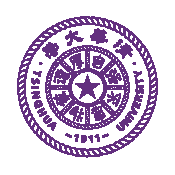
\includegraphics[height=3cm]{thu-fig-logo}}%
  \hspace{4em}%
  \subcaptionbox{第二个小图形,注意这个图略矮些。如果标题很长的话,它会自动换行\label{fig:subfig2}}
      {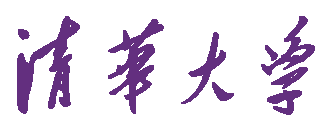
\includegraphics[height=2cm]{thu-text-logo}}
  \caption{包含子图形的大图形(subcaptionbox示例)}
  \label{fig:big1-subcaptionbox}
\end{figure}
\begin{figure}[h]
  \centering%
  \begin{subfigure}{3cm}
    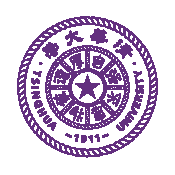
\includegraphics[height=3cm]{thu-fig-logo}
    \caption{第一个小图形}
  \end{subfigure}%
  \hspace{4em}%
  \begin{subfigure}{0.5\textwidth}
    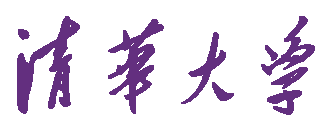
\includegraphics[height=2cm]{thu-text-logo}
    \caption{第二个小图形,注意这个图略矮些。subfigure中同一行的子图在顶端对齐。}
  \end{subfigure}
  \caption{包含子图形的大图形(subfigure示例)}
  \label{fig:big1-subfigure}
\end{figure}

古之学者必有师。师者,所以传道受业解惑也。人非生而知之者,孰能无惑?惑而不从师,
其为惑也,终不解矣。生乎吾前,其闻道也固先乎吾,吾从而师之;生乎吾後,其闻道也亦
先乎吾,吾从而师之。吾师道也,夫庸知其年之先後生於吾乎!是故无贵无贱无长无少,道
之所存,师之所存也。

嗟乎!师道之不传也久矣,欲人之无惑也难矣。古之圣人,其出人也远矣,犹且从师而问焉;
今之众人,其下圣人也亦远矣,而耻学於师。是故圣益圣,愚益愚。圣人之所以为圣,愚
人之所以为愚,其皆出於此乎?爱其子,择师而教之,於其身也,则耻师焉,惑焉。彼童子
之师,授之书而习其句读者,非吾所谓传其道、解其惑者也。句读之不知,惑之不解,或师
焉,或不焉,小学而大遗,吾未见其明也。巫医、乐师、百工之人不耻相师,  士大夫之族
曰“师”曰“弟子”之云者,则群聚而笑之。问之,则曰:彼与彼年相若也,道相似也,位
卑则足羞,官盛则近谀。呜呼!师道之不复,可知矣。巫医、乐师、百工之人。吾子不齿,
今其智乃反不能及,其可怪也欤!圣人无常师。孔子师郯子、苌子、师襄、老聃。郯子之徒,
其贤不及孔子。孔子曰:“三人行,必有我师。”是故弟子不必不如师,师不必贤於弟子。
闻道有先後,术业有专攻,如是而已。

如果要把编号的两个图形并排,那么小页就非常有用了:
\begin{figure}
\begin{minipage}{0.48\textwidth}
  \centering
  
\includegraphics[height=2cm]{thu-whole-logo}
  \caption{并排第一个图}
  \label{fig:parallel1}
\end{minipage}\hfill
\begin{minipage}{0.48\textwidth}
  \centering
  
\includegraphics[height=2cm]{thu-whole-logo}
  \caption{并排第二个图}
  \label{fig:parallel2}
\end{minipage}
\end{figure}

李氏子蟠,年十七,好古文、六艺,经传皆通习之,不拘於时,学於余。余嘉其能行古
道,作师说以贻之。

\hfill —— 韩愈(唐)

\chapter{基于集中平台的iBGP系统结构}
\label{cha:architecture}


\section{本章引言}
可扩展问题是互联网iBGP协议的重要问题,随着网络规模和需求的不断增加,大多数自治系统已经不采用传统的Full-mesh的iBGP连接结构,而是使用配置比较方便、技术比较成熟的路由反射。现有的解决iBGP可扩展问题的思路可分为两种:分布式路由体系结构、集中式路由体系结构。分布式路由体系结构下的相关研究主要有路由反射和AS联邦,其解决了iBGP的可扩展问题,但是带来了新的问题,比如:非最优出口、转发环路、路由震荡。而集中式路由体系结构的相关研究主要有SoftRouter、RCP、RFCP三种代表性方案,这三种方案解决了iBGP的可扩展问题,但也分别存在集中平台本身的可扩展性差、路由存储冗余重复、未优化的传统路由计算方式等等问题。

本文基于数据平面和控制平面分离的思想,提出了基于集中平台的iBGP系统结构,将自治系统内部的路由存储、策略管理、路由计算以及路由转发交换功能合理划分为集中平台和自治系统内边界路由器上执行的两部分。该基于集中平台的iBGP系统结构处理路由信息的基本流程为:
\begin{itemize}
  \item 自治系统内的边界路由器从某eBGP邻居收到路由信息,如果本地路由器配置了需要保存从该邻居过来的路由信息,则保存该路由信息到Adj-RIB-In。经过入站策略后,将过滤更新的路由通过iBGP协议将其发送到集中平台;
  \item 集中平台将收到的路由信息存入Loc-RIB、为每台自治系统内的边界路由器计算出最优路由,将最优路由通过iBGP协议发送给边界路由器;
  \item 每台边界路由器收到集中平台的最优路由,进行出站过滤,边界路由器将收到的路由信息通过eBGP连接宣告给所有的eBGP邻居。如果本地路由器配置了需要保存向某邻居宣告的路由信息,则将向外宣告的路由存入邻居对应的Adj-RIB-Out。
\end{itemize}

\begin{figure}
  \centering
  % Requires \usepackage{graphicx}
  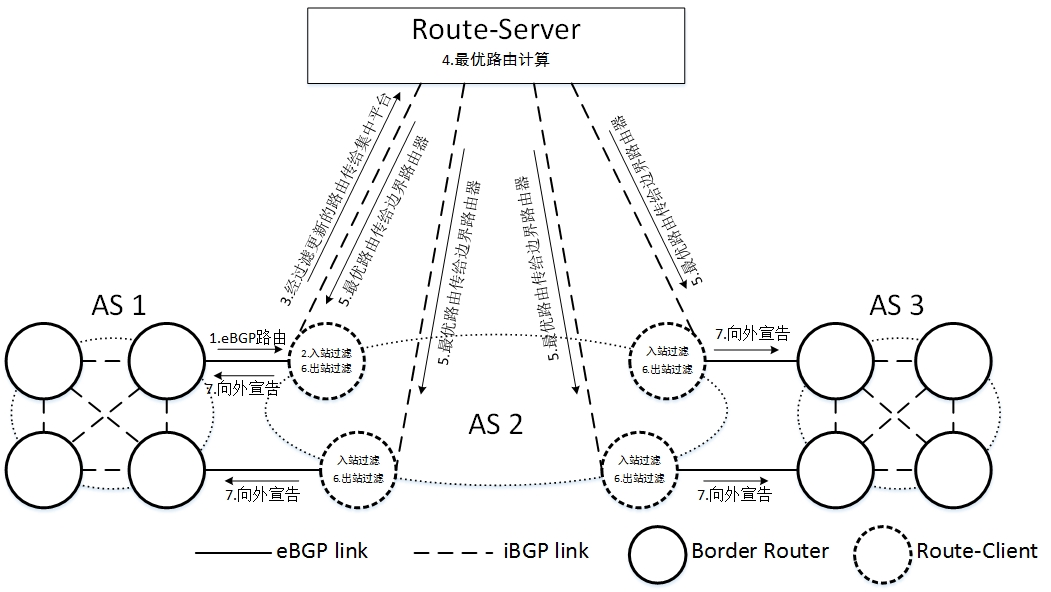
\includegraphics[width=\textwidth]{rscp-ibgp1}
  \caption{RSCP-iBGP系统逻辑架构图}
  \label{fig:rscp-ibgp1}
\end{figure}

集中式路由体系结构下,路由存储、策略管理、路由计算等存在很多优化空间。本文提出的基于集中平台的iBGP系统,不仅解决了iBGP存在的可扩展问题,而且对自治系统内BGP的路由存储和路由计算进行了优化。

本章首先提出基于集中平台的iBGP系统架构,之后对系统中的两个主要模块增量路由存储、复式路由计算进行详细的介绍,最后主要从解决iBGP可扩展问题、与分布式路由体系结构方案的对比、与集中式路由体系结构方案的这三个方面对基于集中平台的iBGP系统进行定性的对比分析。








\section{新型iBGP路由系统}
本文提出的自治系统内部的基于集中平台的iBGP新架构命名为RSCP-iBGP(Route Server Control Platform iBGP)。RSCP-iBGP基本思想是将自治系统内边界路由器的控制平面和数据平面进行部分分离,将边界网关协议BGP中的路由计算、路由存储从边界路由器中剥离出来,交由独立的、且逻辑比较集中的运行在路由控制平台的Route-Server执行,而自治系统内部的普通边界路由器作为Route-Client对路由信息进行接收转发、入站出站过滤更新等操作。

RSCP-iBGP逻辑系统如图\ref{fig:rscp-ibgp1},这个系统运行在自治系统内部,主要包含三部分:自治系统内部的路由控制平台(Route-Server),自治系统内部的多台边界路由器(Route-Client),以及自治系统内部边界路由器与路由控制平台的标准通信接口(iBGP协议),具体流程如图\ref{fig:rscp-ibgp}:
\begin{itemize}
  \item 通信协议使用iBGP协议,来传输BGP路由信息;
  \item 路由控制平台上运行1台Route-Server进行集中式的路由存储、路由计算。当Route-Server收集路由模块,收集到自治系统内部边界路由器Route-Client-Ri发来的更新路由消息,Route-Server现将该路由加入对应的Adj-RIB-In表,之后该路由经过Route-Client-Ri的入站策略后进入Loc-RIB增量存储模块,存储经过入站策略的路由信息,将Loc-RIB表以及IGPcost值输入路由复式计算模块,得到自治系统每台边界路由的针对该前缀的最优路由,之后在路由集中控制平台上分别经过每台边界路由器的出站策略,更新每台边界路由器对应的Adj-RIB-Out表,将其结果输入到分发路由模块,分发路由模块则分别将经过出站策略的该前缀的最优路由传输给自治系统内的每台边界路由;
  \item 自治系统内部的边界路由器Route-Client:
        \begin{itemize}
          \item 当收到其他自治系统发来的eBGP路由时,根据收到路由eBGP邻居的配置,决定是否将其存储到对应eBGP邻居的Adj-RIB-In。边界路由器Route-Client将收到的路由信息进行入站策略的过滤更新,将得到的路由通过iBGP协议发送给路由控制平台上的Route-Server;
          \item 当收到路由控制平台上的Route-Server发来的iBGP路由时,边界路由器Route-Client将收到的路由信息进行出站策略的过滤更新,将经过出战策略的路由其宣告给自己的所有eBGP邻居,同时根据对应的eBGP邻居的配置,决定是否将其存储到对应eBGP邻居的Adj-RIB-Out。
        \end{itemize}
\end{itemize}

\begin{figure}
  \centering
  % Requires \usepackage{graphicx}
  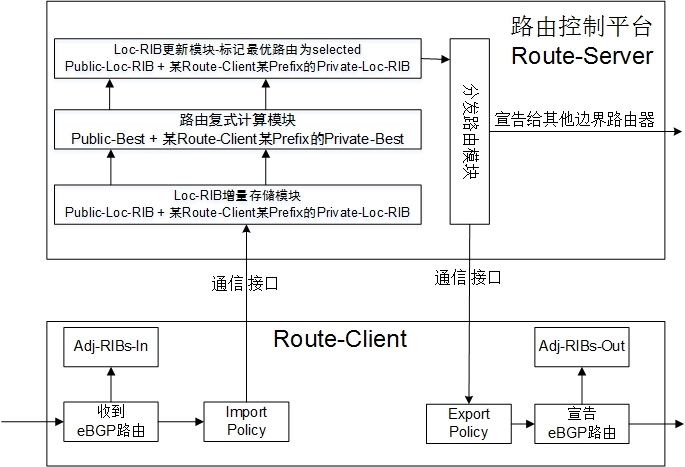
\includegraphics[width=\textwidth]{rscp-ibgp}
  \caption{RSCP-iBGP系统流程模块图}
  \label{fig:rscp-ibgp}
\end{figure}

\section{系统详细介绍}
\subsection{集中平台}
\subsubsection{Loc-RIB增量存储模块}

\begin{figure}
  \centering
  % Requires \usepackage{graphicx}
  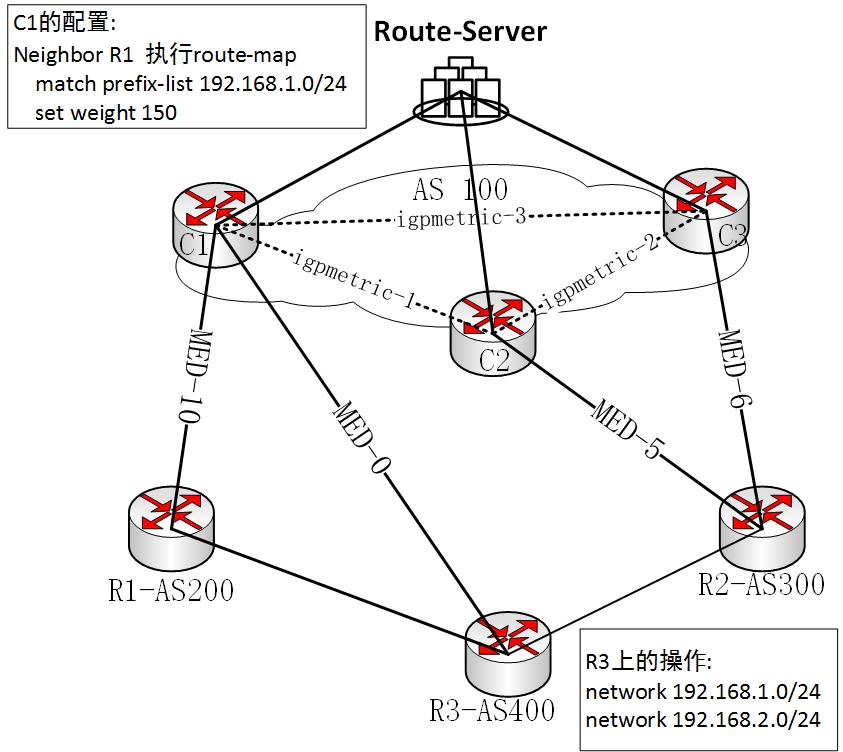
\includegraphics[width=0.75\textwidth]{rscp-example1}
  \caption{Loc-RIB增量存储案例使用的网络拓扑图}
  \label{fig:rscp-example1}
\end{figure}

传统网络中,自治系统的边界路由器收到从eBGP邻居传来的更新路由信息,该边界路由器会将该路由信息经过入站策略后更新到Loc-RIB表,选择最优路由宣告给其iBGP邻居。早期自治系统内的边界路由器建立Full-mesh的iBGP连接,以此来使得外界的路由信息传输到自治系统内部的每台边界路由器。路由经过入站策略后,可能传输到每台边界路由器会有所差异,但大部分前缀在大部分边界路由器上的Loc-RIB表的路由信息都基本相同,入站策略和出站策略主要用于eBGP路由的过滤更新,传统的iBGP策略大多仅配置next-hop-self。根据BGP协议的特性以及网络中路由表的存储实现,本文提出了Loc-RIB增量存储的概念。

综合本文第二章\ref{cha:review}对BGP的路由策略、路由计算的综述,我们会发现对于特定的前缀,在自治系统内的决定每台边界路由器与其他边界路由器最优路由不同的主要原因在2个路由属性Weight和IGPcost:Weight路由属性仅本地路由器有效,不传输给其他的边界路由器;不同边界路由器到其他边界路由器的IGPcost并不相同。仅从路由存储的角度考虑,可以在路由控制平台上的Route-Server中存储一份Public-Loc-RIB,以及在每个iBGP的对等体连接进程中,存储曾配置过Weight值的Prefix的所有路由表项(因为Weight仅在本地路由器有效,并不会影响其他边界路由器的选路,属于边界路由器特有的路由信息,需要单独存储)。Loc-RIB增量存储中增量的含义为,将每台边界路由器特有的路由信息增量存储。为了便于该边界路由器前缀最优路由的计算,将该边界路由器可能受到Weight值影响的前缀的所有路由增量存储。



\begin{table}[h]
	\centering
	\caption{Route-Server上存储的Public-Loc-RIB路由信息}
    \label{tab:weight-example}
	\begin{tabular}{|c|c|c|c|c|c|c|}
		\hline
		network & next-hop & metric & LocPrf & Weight & Path & ebgp-next-hop \\ \hline
		192.168.1.0 & C1 & 0 & &  &400,i & R3 \\ \hline
        192.168.1.0 & C1 & 10 & &  &200,400,i & R1 \\ \hline
        192.168.1.0 & C2 & 5 & &  &300,400,i & R2 \\ \hline
        192.168.1.0 & C3 & 6 & &  &300,400,i & R2 \\ \hline
        192.168.2.0 & C1 & 0 & &  &400,i & R3 \\ \hline
        192.168.2.0 & C1 & 10 & &  &200,400,i & R1 \\ \hline
        192.168.2.0 & C2 & 5 & &  &300,400,i & R2 \\ \hline
        192.168.2.0 & C3 & 6 & &  &300,400,i & R2 \\ \hline
	\end{tabular}
\end{table}

在如图\ref{fig:rscp-ibgp}的拓扑中,ASN(Autonomous System Number,自治系统号)为100的自治系统在部署RSCP-iBGP系统的条件下,在Route-Server中Loc-RIB采用增量存储的方案。AS100中有3台Route-Client作为边界路由器,分别命名为C1、C2、C3。Route-Server存储了C1、C2、C3的路由策略,在集中的路由控制平台上部署了C1的入站策略(C1从R1收到的前缀为192.168.1.0/24的路由将其Weight设置为150)。



\begin{table}[h]
	\centering
	\caption{Route-Server上存储的针对C1的Pravite-Loc-RIB路由信息}
    \label{tab:c1-loc-rib}
	\begin{tabular}{|c|c|c|c|c|c|c|}
		\hline
		network & next-hop & metric & LocPrf & Weight & Path & ebgp-next-hop \\ \hline
		192.168.1.0 & C1 & 0 & &  &400,i & R3 \\ \hline
        192.168.1.0 & C1 & 10 & & 150 &200,400,i & R1 \\ \hline
        192.168.1.0 & C2 & 5 & &  &300,400,i & R2 \\ \hline
        192.168.1.0 & C3 & 6 & &  &300,400,i & R2 \\ \hline
	\end{tabular}
\end{table}

当R3向外宣告两条路由192.16.1.0/24和192.168.2.0/24,Route-Server收到了C1、C2、C3转发过来的路由信息,其存储的Public-Loc-RIB如表\ref{tab:weight-example}。因为前缀为192.168.1.0/24的通过C1传输到集中的路由控制平台的两条路由,均需经过C1的入站策略,C1传输过来的ebgp-next-hop为从R1接收到前缀为192.168.1.0/24的路由经过入站策略路由的Weight值被重设为150,其操作可能影响之后的路由决策,则需要单独存储从C1转发过来的192.168.1.0/24的所有路由,其存储的Private-Loc-RIB如表\ref{tab:c1-loc-rib}。


从表\ref{tab:weight-example}、表\ref{tab:c1-loc-rib}可以看出,Loc-RIB的增量更新方案对于减少Loc-RIB表的存储非常有效。如果自治系统内有N台边界路由器,则Route-Server仅需存储1张Loc-RIB表,加m条单独的路由,其占用存储空间的大小直接下降了一个数量级。


\subsubsection{复式路由计算}

传统的路由计算是分布式的路由计算,在每台边界路由器上输入一张Loc-RIB表,通过将更新前缀的全部路由根据更新时间由近到远两两比较,得到最优路由,属于单输入单输出的传统路由计算方法。而复式路由计算方法中,将所有路由器收到的路由信息Public-RIB-In以及多个存储部分前缀的Private-RIB-In作为复式计算的输入,得到针对特定前缀的所有边界路由器的最优路由,属于多输入多输出的路由计算。

复式路由计算方法的基本思想:因为某些Route-client的某些Prefix的最优路由结果受到Weight值的影响而被单独存储,则遍历所有边界路由器的Private-RIB-In,如果存在该Prefix1,则单独计算该边界路由器的针对该Prefix1的最优路由,并以此结果为准。没有单独存储Prefix1路由的其他边界路由器,针对特定前缀Prefix1,利用Public-RIB-In和IGPcosts, 计算出最优路由。

因为路由计算的过程中可能涉及IGPcosts的比较,我们的复式路由计算算法采用集合缩小法。以前缀Prefix1为例,将其所有的路由加入一个集合,执行以下的步骤,步骤N的输入为步骤(N-1)的输出,直到某一步骤结束后集合仅剩一个元素,即得到了最优路由。假设当路由计算过程在步骤6之后仍没有选出最优路由,之后则针对每台边界路由器单独进行路由计算:

以下步骤,各边界路由器的衡量标准是相同的,可以统一计算:
\begin{itemize}
    \item 步骤1:删除集合中权重(Weight)不是最高的路由信息,留下权重最高的路由信息。
    \item 步骤2:删除集合中本地优先级(Local Preference)不是最高的路由信息,留下本地优先级最高的路由信息。
    \item 步骤3:如果集合中有本地路由器初始的路由(本地初始的路由在BGP表中的下一跳显示为0.0.0.0),则删除其他路由信息。
    \item 步骤4:删除集合中As-path不是最短的路由信息,留下As-path最短的路由信息。
    \item 步骤5:删除源代码(Origin code)不是最小的路由信息,留下源代码最小的路由信息(IGP<EGP<不完整路由)。
    \item 步骤6:删除MED(Multi-Exit Discriminators,多出口鉴别符)不是最低的路径,只有当所有待选路由来自同一AS时(可通过As-path判断),路由器才会对比MED。
\end{itemize}


以下步骤,因为边界路由器两两之间的IGPcost各有不同,所以各边界路由器开始单独计算,即单独执行下列步骤,直到得到最优路由:
\begin{itemize}
    \item 步骤7:优选去往BGP下一跳最短的路径,即删除集合中IGPcost不是最小的路由,留下IGPcost最小的路由。
    \item 步骤8:优选eBGP最老的路由,减少路由反复启动和禁用的风险,即删除集合中eBGP不是最老的路由,留下eBGP最老的路由。
    \item 步骤9:优选eBGP邻居发给Route-Client路由的边界路由器ID值router-id最低的路由(该eBGP邻居的Route-id需传输到集中平台)。
    \item 步骤10:优选从eBGP邻居收到的其路由器IP地址最小的路由(该eBGP邻居的IP地址需传输到集中平台)。
\end{itemize}


自治系统内的边界路由器在iBGP连接中仅将前缀对应的最优路由传输给其iBGP邻居,iBGP邻居收到最优路由后会继续计算最优路由,如果最优路由发生改变则继续传输……,这是自治系统内部的路由收敛过程。当eBGP路由传入自治系统,在全连接的iBGP结构下路径搜索过程计算次数最少N次,最多\verb+N*(N-1)/2+次。而在本文提出的复式路由计算在自治系统内,没有路径搜索和路径收敛的过程,eBGP路由直接从边界路由器传输到路由控制平台Route-Server上,Route-Server有全部的路由信息表,结合图\ref{fig:rscp-ibgp}中的IGP拓扑配置模块(从该模块中获取IGPcost值),由Route-Server为自治系统内的每台边界路由器计算最优路由,计算次数最少1次,最多N次。选择此复式路由模块,当自治系统收到路由更新时,路由计算的总次数至少下降一个数量级。

\subsubsection{路由宣告}
当集中平台收到iBGP邻居的路由宣告,集中平台上的Route-Server经过Loc-RIB增量存储模块和复式路由计算,得到自治系统内所有边界路由器Route-Client的更新路由,Route-Server将更新路由通过扩展的iBGP协议宣告给自治系统内所有的边界路由器Route-client。

\subsection{边界路由器}
传统的运行BGP协议的自治系统内的边界路由器,在路由信息的处理过程中,需要使用三种RIB表,分别是Adj-RIBs-In、Loc-RIB、Adj-RIBs-Out表。在RSCP-iBGP的新架构中,Adj-RIBs-In和Adj-RIBs-Out根据配置文件决定是否进行存储在边界路由器上。

\subsubsection{Adj-RIBs-In}
一般运行BGP协议的路由器默认不存储从邻居获得的所有未经入站策略的路由信息,即默认不存储Adj-RIB-In。如果路由器想要存储从某个BGP邻居收到的所有未经入站策略的路由信息,则需要通过配置文件进行配置,对应的语句为:neighbor [ip-address] soft-reconfiguration inbound,该语句告诉BGP进程保存从指定邻居那里获得的所有更新。


假设自治系统有N台边界路由器Route-Client,Route-Server路由器与这N台Route-Client分别建立N个iBGP连接,如果Route-Server在某个iBGP连接的neighbor配置里面设置了保存收到的所有更新,则Route-Server存储从对应的Route-Client收到的所有未经入站策略的原始路由信息Adj-RIB-In。通过语句show ip bgp neighbors [ip-address] received-routes可以查看Adj-RIB-In。

传统的自治系统Full-mesh的iBGP连接网络中,如果有N台边界路由器均开启了存储Adj-RIB-In的选项,通过域内的路由信息传播收敛过程,Adj-RIBs-In冗余存储了N份全部的路由信息。如果在集中平台上将收到的eBGP路由进行Adj-RIB-In存储,因为没有域内的BGP路由信息传播,则集中平台全部是我Adj-RIBs-In仅存储了1份全部的路由信息,极大的节省了存储空间。


\subsubsection{Adj-RIBs-Out}
一般运行BGP协议的路由器默认不存储经过出站策略准备宣告给邻居的路由信息,即默认不存储Adj-RIBs-Out。如果路由器想要存储经过出站策略准备宣告给邻居的路由信息,则需要通过配置文件进行配置,对应的语句为:neighbor [ip-address] soft-reconfiguration outbound,该语句告诉BGP进程保存向指定邻居那里宣告的所有更新。


假设自治系统有N台边界路由器Route-Client,Route-Server路由器与这N台Route-Client分别建立N个iBGP连接,如果Route-Server在某个iBGP连接的neighbor配置里面设置了保存向外宣告的所有更新,则Route-Server存储从对应的Route-Client宣告给邻居的所有路由信息。通过语句show ip bgp neighbors [ip-address] advertised-routes可以查看Adj-RIB-Out。

传统的自治系统Full-mesh的iBGP连接网络中,如果有N台边界路由器均开启了存储Adj-RIB-Out的选项,通过域内的路由信息传播收敛过程,每份Adj-RIB-Out均需存储了1份每一个前缀对应的最优路由信息。如果在集中平台上将经过过滤的发放给每台边界路由器,用于eBGP宣告的最优路由进行Adj-RIB-Out存储,则集中平台每份Adj-RIB-Out也均需存储了1份每一个前缀对应的最优路由信息。


\subsubsection{路由宣告}

当自治系统内的边界路由器Route-Client收到eBGP邻居的路由更新,路由信息在边界路由器Route-Client经过入站策略,将路由信息通过扩展的iBGP路由协议(路由信息中传输路由属性Weight)传输到集中平台Route-Server。

当自治系统内的边界路由器Route-Client收到iBGP邻居(集中平台的Route-Server)的路由更新,路由信息在边界路由器Route-Client经过出站策略,将路由信息通过eBGP路由协议传输其他的自治系统。

\begin{figure}
  \centering
  % Requires \usepackage{graphicx}
  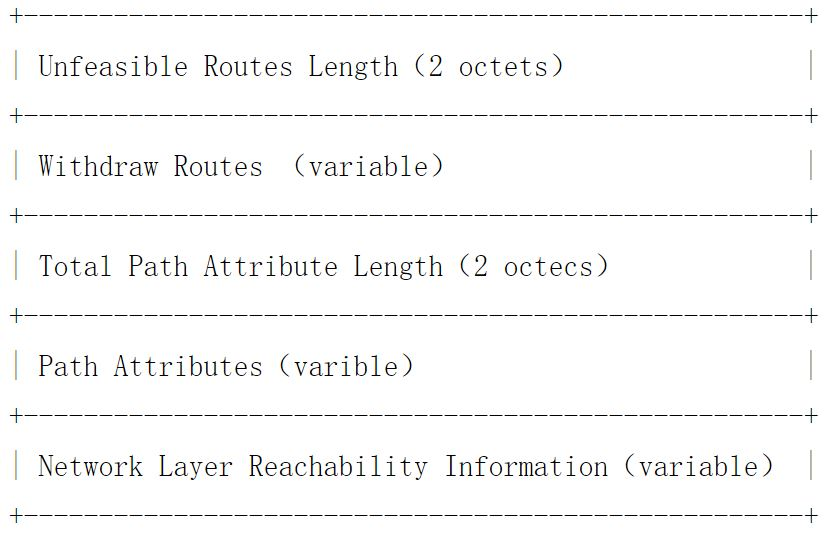
\includegraphics[width=0.6\textwidth]{updatemsg}
  \caption{UPDATE消息数据格式}
  \label{fig:updatemsg}
\end{figure}



\subsection{扩展的iBGP路由协议}
路由信息通过UPDATE消息在路由器之间进行传输。在本文提出的基于集中平台的iBGP新架构RSCP-iBGP中,需要将经过边界路由器Route-Client上的入站策略的路由信息传输到集中平台的Route-Server,包括路由信息中原本不在自治系统间传输的路由属性Weight,所以需要对自治系统内边界路由器上运行的BGP协议进行扩展:增加Path Attributes,从而能在自治系统内部通过扩展的iBGP协议传输附带Weight属性值的UPDATE路由信息。

BGP报文消息\cite{rfc4271}基于TCP协议进行传输,BGP消息主要由BGP头和数据部分组成。BGP消息报文的最大长度是4096字节,最小是只包含BGP头没有数据仅19字节。BGP头部的长度为19字节,主要包含Marker、Length、Type三种类型的数据。BGP头部的Type字段主要标记BGP消息的类型:Type值为1表示OPEN消息,Type值为2表示UPDATE消息,Type值为3表示NOTIFICATION消息,Type值为4表示KEEPALIVE消息。

UPDATE消息主要用于BGP对等体之间宣告可达路由或者撤销不可达路由。BGP协议的UPDATE消息主要包含19字节的BGP头以及变长的UPDATE消息数据, 如图\ref{fig:updatemsg}。Path Attributes字段中记录了路由信息的属性,该字段由一个三元组组成<attribute type, attribute length, attribute value>。Attribute Type字段包含两部分Flag和Type Code。 Flag的长度为1个字节,前4位比特位取0或1,分别代表公认属性或可选属性、非传递属性或可传递属性、信息完整或信息不完整、属性长度为1字节或属性长度为2字节。已有的路径属性中的典型Type Code取值从1-7,分别对应路由信息的起源Origin、自治系统路径编号、Next\_hop值、MED属性值、Local Preference值、Atomic\_aggregate、Aggregate。

为了在自治系统间的iBGP连接中传输Weight属性,本文对Path Attributes的Attribute Type进行扩展,以下对传输Weight属性的Path Attribute三元组中设计的元素进行设计:
\begin{itemize}
  \item Flag为01000000,表示Weight属性为公认属性则所有路由器均可识别,Weight属性为可传递属性,在RSCP-iBGP系统中需要从边界路由器传输到集中平台,信息是完整的,且属性长度是1字节;
  \item 设计传输Weight属性的Attribute Type Code为31(本文提出的RSCP-iBGP系统基于Quagga\cite{quagga}实现,目前Quagga中BGP协议实现的Attribute Type Code没有值为31的Path Attribute);
  \item Weight属性值的范围为 0-$(2^{16}-1)$,则传输Weight的Attribute Length值为2,转为16进制为0x02。
\end{itemize}

\section{对比分析}

为了解决iBGP可扩展问题,学术界提出了分布式路由体系结构下的路由反射和AS联邦,以及集中式路由体系结构下的SoftRouter、RCP、RFCP等5种解决方案。其5种方案虽然很好地解决了iBGP存在的可扩展问题,但存在新的隐患,比如路由反射、AS联邦带来的非最优路由、路由震荡等,也没有充分利用新方案的结构优势,比如SoftRouter、RCP以及RFCP并没有对路由存储和路由计算进行优化等。本文提出的RSCP-iBGP系统不仅解决了iBGP可扩展问题,且解决了现有的分布式路由体系结构方案存在的非最优路由、路由震荡等问题,优化了现有集中式路由体系结构方案没有优化的路由存储和路由计算,具体的理论分析如下。

\begin{figure}
  \centering
  % Requires \usepackage{graphicx}
  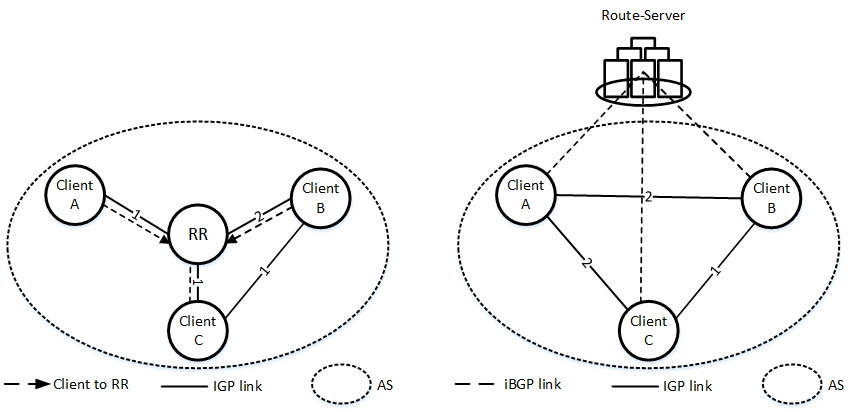
\includegraphics[width=0.75\textwidth]{rscp-best}
  \caption{解决路由反射引起的非最优出口举例}
  \label{fig:rscp-best}
\end{figure}


\subsection{解决iBGP可扩展问题}

假设某自治系统有N台边界路由器,在传统Full-mesh的iBGP结构中,域内自治系统需要建立\verb+N*(N-1)/2+数量的BGP连接。该自治系统的拓扑结构对应到本文的RSCP-iBGP系统结构,自治系统内的有N台Route-client边界路由器用于接受转发其他自治系统传输过来的路由、1台或者多台运行在路由控制平台的Route-Server用于路由存储和路由计算等操作,N台Route-Client与1台Route-Server建立N个iBGP连接来传输BGP路由信息。iBGP连接数量下降了一个数量级,则该基于集中平台的RSCP-iBGP新架构解决了iBGP协议可扩展性差的问题。

\subsection{与分布式路由体系结构方案的对比}

学术界提出的2种比较典型的分布式路由体系结构方案分别是路由反射和AS联邦,具体的概念和存在的问题在第二章进行了详细的综述,本文提出的RSCP-iBGP系统没有路由反射中非最优出口、转发环路、路由震荡等问题,也没有AS联邦中非最优出口和路由震荡等问题。

\subsubsection{解决路由反射存在问题}



路由反射在特定情况下,因为最优路由计算缺少全部路由、结构设计不合理、MED值不可比等多方面原因,可能产生非最优路由、转发环路、路由震荡等问题。但在本文的RSCP-iBGP新系统中,路由计算基于全部的路由信息,不存在路由反射器将最优路由发送给客户机作为客户机最优路由的设计,采用集合缩小法统一比较而不是两两比较的路由算法解决了MED值不可比的问题,所以RSCP-iBGP新系统解决了路由反射的非最优路由、转发环路和路由震荡的问题,对比章节\ref{subsubsec:rr}的例子具体说明。\\

\begin{figure}
  \centering
  % Requires \usepackage{graphicx}
  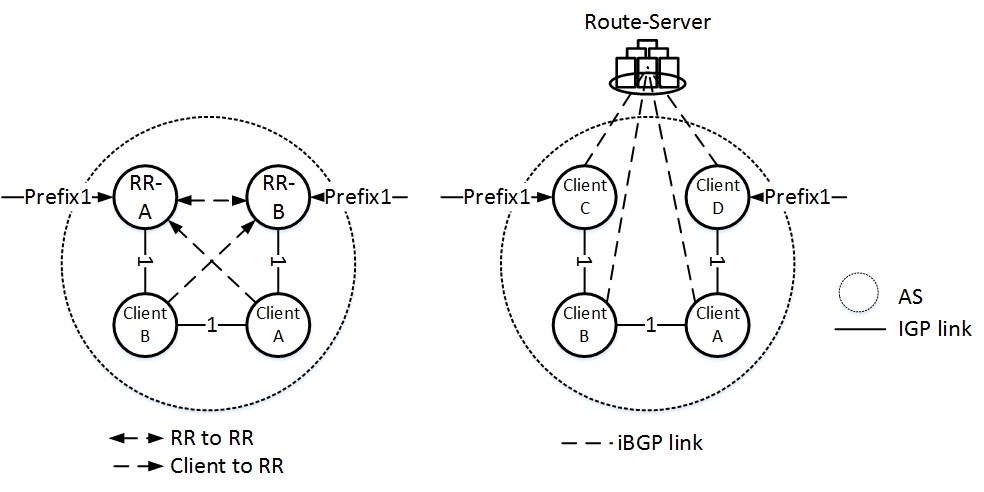
\includegraphics[width=0.9\textwidth]{rscp-noloop}
  \caption{解决路由反射引起的转发环路举例}
  \label{fig:rscp-noloop}
\end{figure}

在图\ref{fig:rscp-best}中,左侧为路由反射自治系统内的网络结构,右侧为RSCP-iBGP新系统下自治系统内的网络结构。Client-A和Client-B分别接收到一条eBGP路由,其来自同一AS,且前缀、Weight、Local Preference、As-path、MED值均相同。在RSCP-iBGP新系统中,Client-A和Client-B会将这两条路由传输到路由控制平台Route-Server;Route-Server通过复式路由计算为自治系统内的3个边界路由器计算最优路由,因为这两条路由来自同一AS,且前缀、Weight、Local Preference、As-path、MED值均相同,则根据IGPcost进行路由选择,Client-A选择自己接收到eBGP路由作为该前缀的最优路由,Client-B选择自己接收到eBGP路由作为该前缀的最优路由,Client-C选择Client-B作为自己的最优出口,即Client-C选择client-B从eBGP邻居收到的路由作为自己的最优路由。

RSCP-iBGP新系统解决了路由反射中的非最优路由问题,因为RSCP-iBGP新系统上所有边界路由器的最优路由计算都是基于全部的路由信息,所以计算结果均是理论上的最优路由。\\




章节\ref{subsubsec:rr}中路由反射转发环路发生的原因是路由反射结构设置不合理,数据包在转发的过程中多次被重新路由。在RSCP-iBGP新系统中,如图\ref{fig:rscp-noloop},Client-C(对应路由反射器RR-A)和Client-D(对应路由反射器RR-B)会将其收到的路由信息传输给路由控制平台上的Route-Server,Client-C收到的路由记为Prefix1-route1, Client-D收到的路由标记为Prefix1-route2,Route-Server会经过复式路由计算模块计算出自治系统内的四台边界路由器的最优路由,Client-B的最优出口是Client-C,Client-A的最优出口是Client-D。当Client-B要发送目的地址为Prefix1的数据包时,直接通过Client-C转发出去,不会发生路由环路。\\

\begin{figure}
  \centering
  % Requires \usepackage{graphicx}
  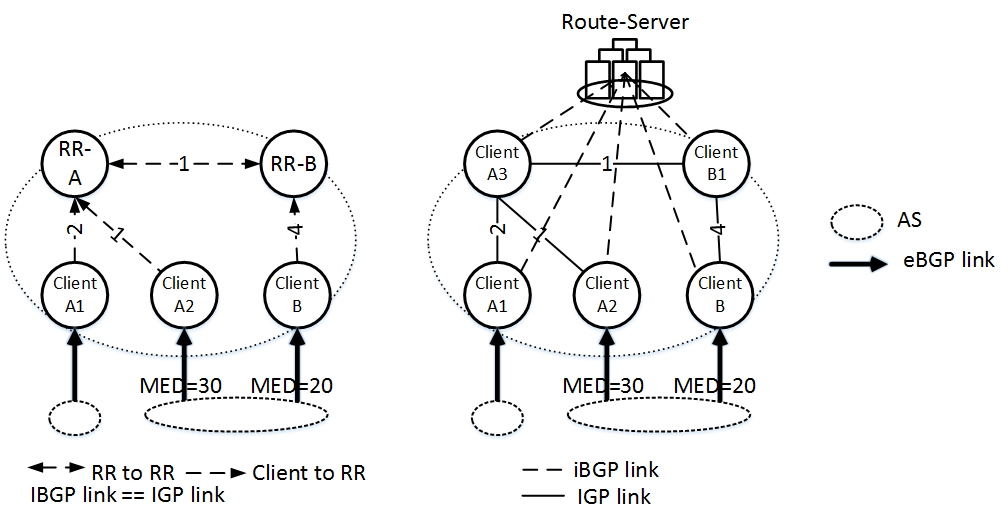
\includegraphics[width=0.9\textwidth]{rscp-nomed}
  \caption{解决路由反射引起的MED路由震荡举例}
  \label{fig:rscp-nomed}
\end{figure}



路由反射引起的MED震荡主要是因为某些时候MED值不可比较,导致最优路由的结果变化,从而发生路由震荡。在图\ref{fig:rscp-nomed}中,左侧为章节\ref{subsubsec:rr}中路由反射结构中因为MED值发生路由震荡的网络结构,右侧为左侧对应的RSCP-iBGP新系统下自治系统内的网络结构。在RSCP-iBGP的新系统中,Client-A1、Client-A2、Client-B收到的3条路由均会传输到路由控制平台的Route-Server。因为传输到自治系统内的3条路由,前缀、Weight、Local Preference、As-path长度均相同。Route-Server的复式路由计算模块,采用集合缩小法,对于域内的所有边界路由器,Client-B收到的eBGP路由优于Client-A2收到的eBGP路由,所以自治系统内的其他路由器的最优路由,根据IGPcost,在client-A1收到的eBGP路由和Client-B收到的eBGP路由,这两条路由之间选择。在RSCP-iBGP新系统中,路由计算采用集合缩小法,基于全部的路由进行路由计算,并不会因为MED值产生路由信息震荡。\\


\begin{figure}
  \centering
  % Requires \usepackage{graphicx}
  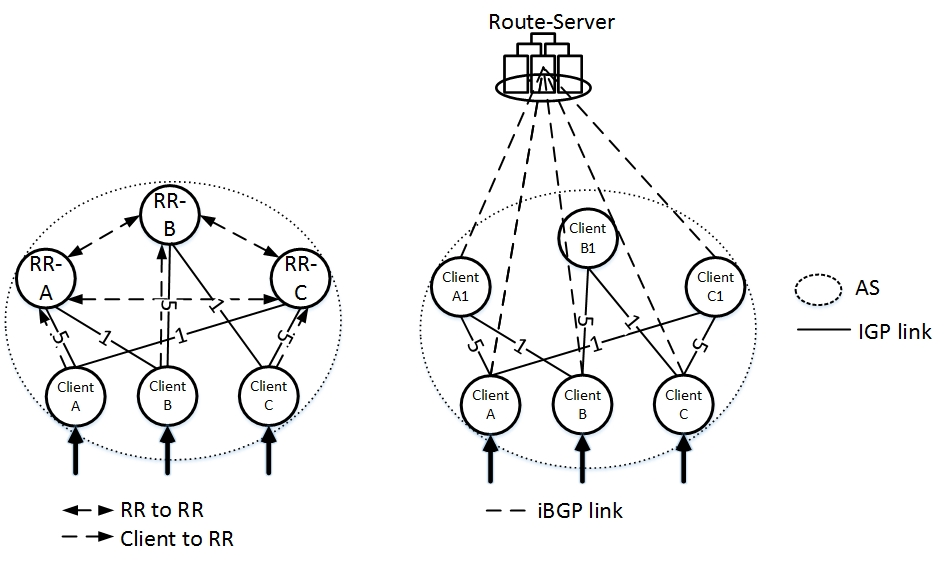
\includegraphics[width=0.9\textwidth]{rscp-notopo}
  \caption{解决路由反射引起的拓扑路由震荡举例}
  \label{fig:rscp-notopo}
\end{figure}


路由反射引起的拓扑震荡主要是因为路由反射结构设计不合理,路由决策主要依赖IGPcost值,一旦接收到其他路由反射器的最优路由,自己本身的最优路由会发生改变,将本身的最优路由宣告出去之后,会引起其他路由反射器最优路由的变化,最终导致路由震荡产生。在图\ref{fig:rscp-notopo}中,左侧为章节\ref{subsubsec:rr}中路由反射结构中因为路由反射结构设计不合理发生路由震荡的网络结构,右侧为左侧对应的RSCP-iBGP新系统下自治系统内的网络结构。在RSCP-iBGP的新系统中,Client-A、Client-B、Client-C收到的3条路由均会传输到路由控制平台的Route-Server。因为传输到自治系统内的3条路由,前缀、Weight、Local Preference、As-path长度、MED均相同,则在Route-Server的复式路由计算模块中,主要依据IGPcost计算自治系统内的所有边界路由器的最优路由,Client-A1的最优出口是Client-B,Client-B1的最优出口是Client-C,Client-C1的最优出口是Client-A。在RSCP-iBGP新系统中,基于全部路由进行路由计算,解决了路由反射因为路由反射器仅反射最优路由的特性以及Cluster结构、路由反射拓扑设计等导致的路由震荡。

\subsubsection{解决AS联邦存在问题}


\begin{figure}
  \centering
  % Requires \usepackage{graphicx}
  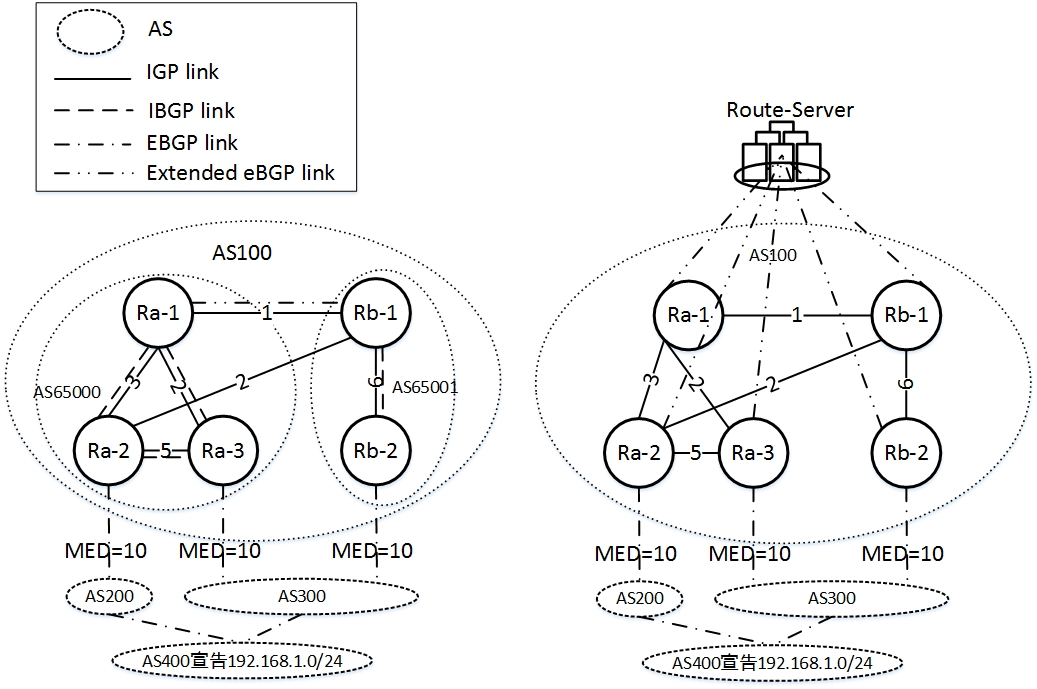
\includegraphics[width=0.9\textwidth]{rscp-asbest}
  \caption{解决AS联邦引起的非最优路由举例}
  \label{fig:rscp-asbest}
\end{figure}

AS联邦解决了iBGP可扩展问题,但在特定情况下也会产生路由计算非最优路由、路由震荡等问题。本文提出的RSCP-iBGP新系统,路由计算基于全部的路由信息,同时为全部边界路由器计算最优路由,没有路由收敛的过程,不会出现AS联邦存在的隐患。\\

AS联邦导致的非最优路由主要原因,在于自治系统内部的子自治系统之间仅传输最优路由,这直接导致某些子自治系统并没有全部的路由信息。在图\ref{fig:rscp-asbest}中,左侧为章节\ref{subsubsec:rr}中AS联邦结构中产生非最优路由情况的网络拓扑,右侧为左侧对应的RSCP-iBGP新系统下自治系统内的网络结构。在RSCP-iBGP的新系统中,Ra-2、Ra-3、Rb-2收到的3条由自治系统400向外宣告的192.168.1.0/24的路由信息,这3条路由信息均会传输到路由控制平台的Route-Server。因为传输到自治系统内的3条路由,前缀、Weight、Local Preference、As-path长度、MED均相同,则在Route-Server的复式路由计算模块中,主要依据IGPcost计算自治系统内的所有边界路由器的最优路由,Ra-1的最优出口是Ra-3,Rb-1的最优出口是Ra-2。在RSCP-iBGP新系统中,基于全部路由进行路由计算,解决了AS联邦的非最优路由问题。\\




\begin{figure}
  \centering
  % Requires \usepackage{graphicx}
  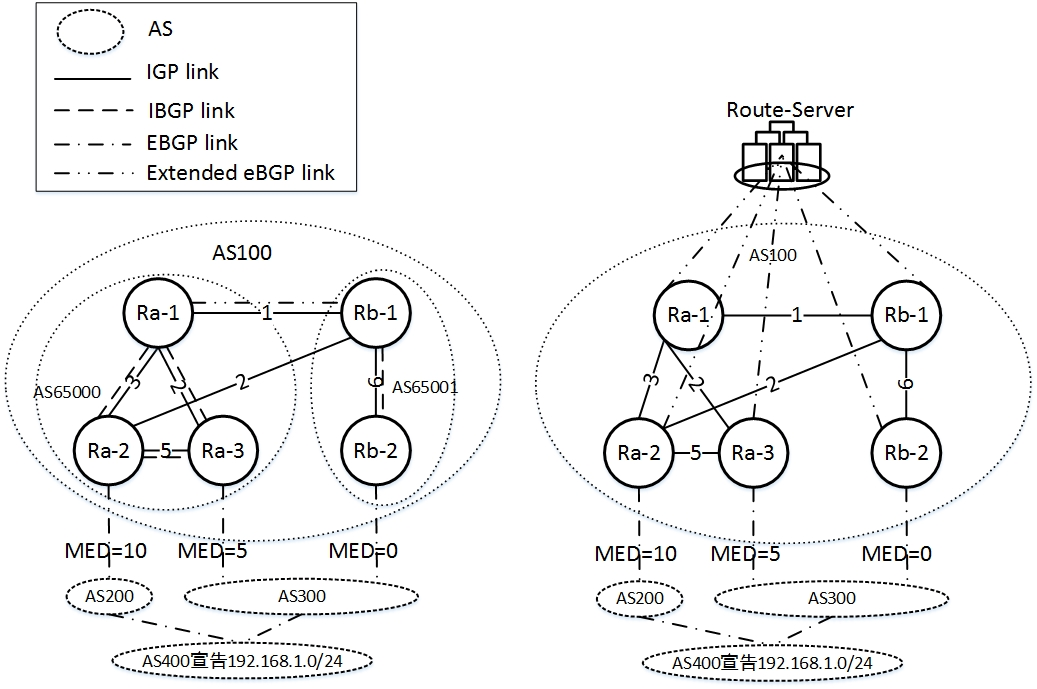
\includegraphics[width=0.9\textwidth]{rscp-asnomed}
  \caption{解决AS联邦引起的路由震荡举例}
  \label{fig:rscp-asnomed}
\end{figure}


AS联邦导致的路由震荡主要原因,在于自治系统内部的子自治系统之间仅传输最优路由,且最优路由两两比较中MED不可比,这直接导致某些子自治系统向外宣告的最优路由会随着接收到的新的路由信息产生变化,最后在路由收敛的过程中产生路由震荡。在图\ref{fig:rscp-asnomed}中,左侧为章节\ref{subsubsec:rr}中AS联邦结构中产生路由震荡的网络拓扑,右侧为左侧对应的RSCP-iBGP新系统下自治系统内的网络结构。在RSCP-iBGP的新系统中,Ra-2、Ra-3、Rb-2收到的3条由自治系统400向外宣告的192.168.1.0/24的路由信息,这3条路由信息均会传输到路由控制平台的Route-Server。因为传输到自治系统内的3条路由,前缀、Weight、Local Preference、As-path长度均相同,则在Route-Server的复式路由计算模块中,主要依据MED、IGPcost等计算自治系统内的所有边界路由器的最优路由。Route-Server的复式路由计算模块,采用集合缩小法,对于域内的所有边界路由器,Rb-2收到的eBGP路由优于Ra-3收到的eBGP路由,所以自治系统内的其他路由器的最优路由,主要根据IGPcost,在Ra-2收到的eBGP路由和Rb-2收到的eBGP路由,这两条路由之间选择。Ra-1的最优出口是Ra-2,Rb-1的最优出口是Ra-2,Ra-3的最优出口是Ra-2。在RSCP-iBGP新系统中,基于全部路由进行路由计算,且没有路由收敛的过程,解决了AS联邦的路由震荡问题。

\subsection{与集中式路由体系结构方案的对比}


学术界提出的3种比较典型的集中式路由体系结构方案分别是SoftRouter、RCP、RFCP,具体的概念和存在的问题在第二章进行了详细的综述,本文提出的RSCP-iBGP系统借鉴了集中式路由体系结构的概念,充分利用集中平台的资源和优势,对路由存储和路由计算进行了优化。

\subsubsection{SoftRouter}

本文提出的RSCP-iBGP新系统的结构,相对于SoftRouter中CE和FE多对多的结构要简单很多,其平台本身的可扩展性要比SoftRouter要好;SoftRouter中对路由存储和路由计算并没有进行优化,主要思想是将其控制平面与数据平面分离,而RSCP-iBGP新系统中对路由存储、路由计算都进行了优化,均优化了一个数量级单位的指标;SoftRouter容易开发部署新的功能,而本文提出的RSCP-iBGP拥有集中平台这一显著优势,也能充分利用集中平台的资源,在集中平台上部署更多的网络功能,加强路由协议的安全性以及配置路由策略的灵活性等等。

\subsubsection{RCP}
RCP路由控制平台提出了集中式路由存储、策略配置、路由计算的思想,不仅在自治系统内部有集中控制平台,同时部署了RCP的自治系统之间也能通过RCP的平台进行域间的信息传输。本文提出的RSCP-iBGP新系统,和RCP的基本思想相同,但具体实现有所差异。本文提出的RSCP-iBGP系统平台的可扩展性更强,注重解决iBGP的问题,且在集中式的路由控制平台上实现了路由计算、路由存储的优化。未来RSCP-iBGP也能充分利用集中平台的优势,实现路由策略的配置集中管理和优化、路由配置正确性检测等方案。


\subsubsection{RFCP}

RFCP是集中式收集路由信息,通过构建虚拟的拓扑环境模拟真实自治系统内的网络环境,将虚拟拓扑环境中Full-Mesh的分布式计算结果传输给真实的网络结构。RFCP的实现需要部署SDN的可编程式交换机,在自治系统内的运行SDN控制器上运行应用程序来进行路由计算,集中式的对路由信息进行管理。但其路由表在虚拟的拓扑环境中仍冗余存储,路由计算属于传统的分布式计算方法,策略配置仍需要在每台边界路由器上进行配置。RSCP-iBGP新系统与RFCP相比,存在很多优势,其不仅将路由存储空间和路由计算次数优化了一个数量级的标准,集中平台的优势和资源,也能帮助网络管理员更好地进行路由存储和路由计算。


\begin{table}[h]
	\centering
	\caption{RSCP-iBGP新系统与现有解决iBGP可扩展问题的相关研究的对比}
    \label{tab:compare}
	\begin{tabular}{|l|c|c|c|c|c|c|}
		\hline
		关注点 & RR & AS联邦 & SoftRouter & RCP & RFCP & RSCP-iBGP \\ \hline
		路由可扩展性:不需要全连接 &  $\surd$ &  $\surd$  & $\surd$  &$\surd$ & $\surd$  &$\surd$  \\ \hline
        路由计算:基于全部路由 & $\times$ &  $\times$  & $\surd$  &$\surd$ & $\surd$  &$\surd$  \\ \hline
        路由计算:no MED引起的震荡 &  $\times$ &  $\times$  & $\surd$  &$\surd$ & $\surd$  &$\surd$  \\ \hline
        路由计算次数优化&  $\times$ &  $\times$  & $\times$  &$\times$ & $\times$  &$\surd$  \\ \hline
        路由表集中存储&  $\times$ &  $\times$  & $\surd$  &$\surd$ & $\times$  &$\surd$  \\ \hline
        路由表存储优化&  $\times$ &  $\times$  & $\times$  &$\times$ & $\times$  &$\surd$  \\ \hline
	\end{tabular}
\end{table}

\subsection{总结}

本章节主要论证本文提出的RSCP-iBGP新系统,相比于现有的学术界提出的2种分布式路由体系结构下的方案、3种集中式路由体系结构下的方案具有的优势,以及该方案的设计目标和价值意义。概括性的比较如图\ref{tab:compare}所示。



\section{本章小结}

本文提出的RSCP-iBGP新系统不仅能解决iBGP存在的可扩展问题,还能够在路由计算的过程中基于全部的路由,达到与Full-Mesh结构下的路由信息扩散传输相同的程度。在此基础上,RSCP-iBGP新系统利用集中平台的优势和资源,对传统的分布式的路由存储和路由计算进行了优化,将存储空间以及当存在路由更新时自制系统内的路由计算次数均优化了一个数量级的标准。本章节详细介绍了RSCP-iBGP的系统架构、路由存储和路由计算的优化方案,以及将该系统与现有解决iBGP可扩展研究方案进行了对比分析,论证了该RSCP-iBGP新系统的设计合理性、显著优势等理论。


\chapter{RSCP-iBGP系统的设计实现}
\label{cha:design}

\section{本章引言}
本文基于软件路由器Quagga\cite{quagga}的开源代码,实现了RSCP-iBGP内部域间路由协议系统。该系统主要分三部分:边界路由器Route-Client、集中式的路由控制平台上运行的Route-Server、边界路由器与Route-Server之间的扩展iBGP通信协议。本章首先解释设计实现平台Quagga的概念以及其虚拟软件路由器上BGP的路由功能实现细节,之后详细介绍RSCP-iBGP系统的三个部分边界路由器、路由控制平台、通信接口的具体设计与实现。

\section{设计实现平台Quagga介绍}

\begin{figure}
  \centering
  % Requires \usepackage{graphicx}
  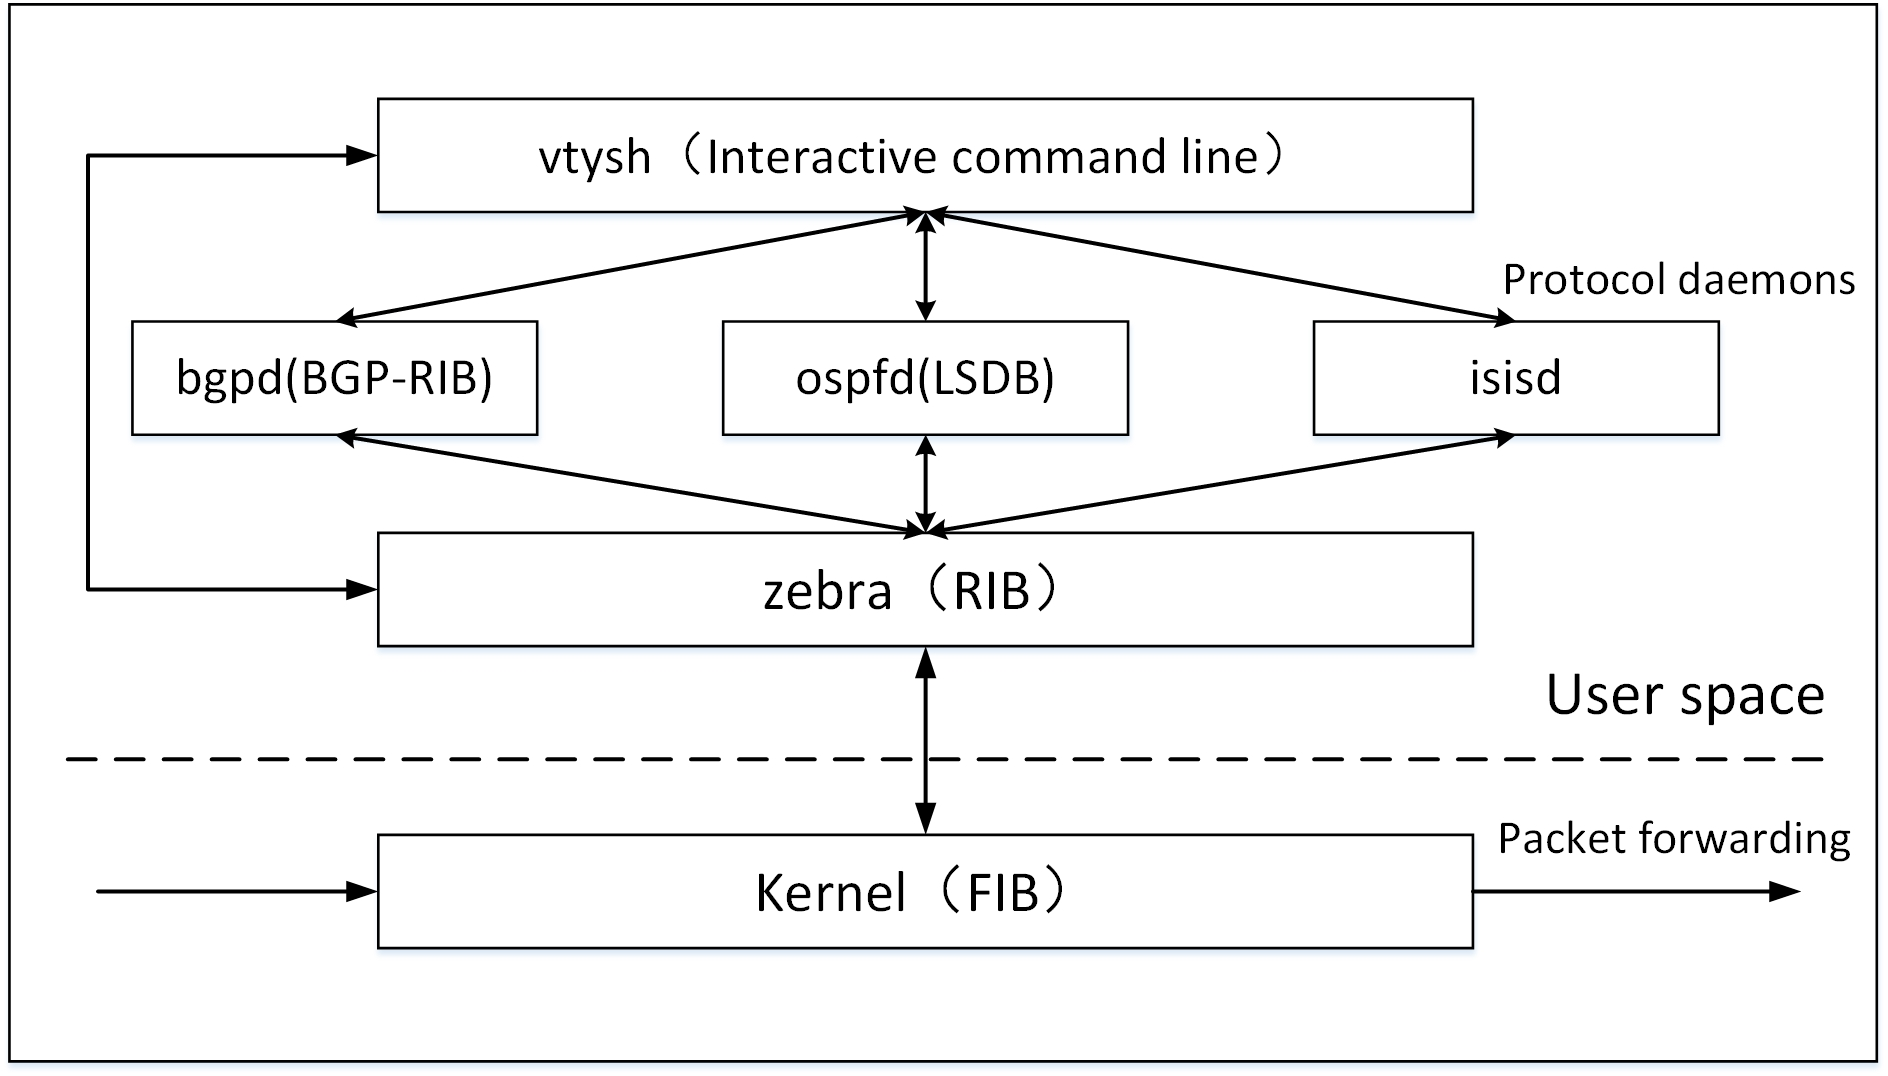
\includegraphics[width=0.75\textwidth]{quagga}
  \caption{Quagga系统结构图\cite{jakma2014quagga}}
  \label{fig:quagga}
\end{figure}


\subsection{基本概念及系统结构}
Quagga是一个比较成熟的虚拟路由器系统,该系统实现了多种网络协议,比如RIPv1、RIPv2、RIPng、OSPFv2、OSPFv3、BGPv4+、IS-IS等。Quagga中不同的网络协议需要运行不同的进程,属于多进程结构,协议之间相互独立,其本身的扩展性、维护性较强 \cite{quaggaThesis}。此外,Quagga中包含一个路由信息管理进程zebra,该进程和各种运行网络协议的进程通过ZServ协议进行交互,将运行网络协议进程产生的有效路由信息安装到内核\cite{jakma2014quagga}。每个协议进程均有自己的配置文件和终端接口,配置不同的网络需要在不同的网络进程内的配置文件中完成,非常麻烦。比如配置BGP网络时,需要在bgpd进程中的配置文件中完成;配置静态路由时,需要在zebra进程中的配置文件中完成。为此,Quagga存在vtysh进程来对Quagga中的其他进程进行配置。vtysh提供一个交互式的命令行接口来输入配置信息,其和其他进程通信通过一个简单的字符串传输协议。在vtysh进程中可以完成网络协议的配置、静态路由配置等对其余每一个进程的配置操作。Quagga的结构如图\ref{fig:quagga}。
\subsection{BGP协议的路由存储}

BGP协议中路由信息表有3种Adj-RIBs-In、Loc-RIB、Adj-RIBs-Out,Quagga中BGP协议的实现在bgpd进程中。bgpd进程中所有的数据结构均存储在bgp\_master结构体中,bgp\_master的成员变量中存在一个链表,包含了所有的bgp实例。每个bgp实例中存储了该BGP session的配置文件、一个链表包含所有的peer实例、静态路由表、路由表(Loc-RIB,结构体为bgp\_table)等信息。


\begin{figure}
  \centering
  % Requires \usepackage{graphicx}
  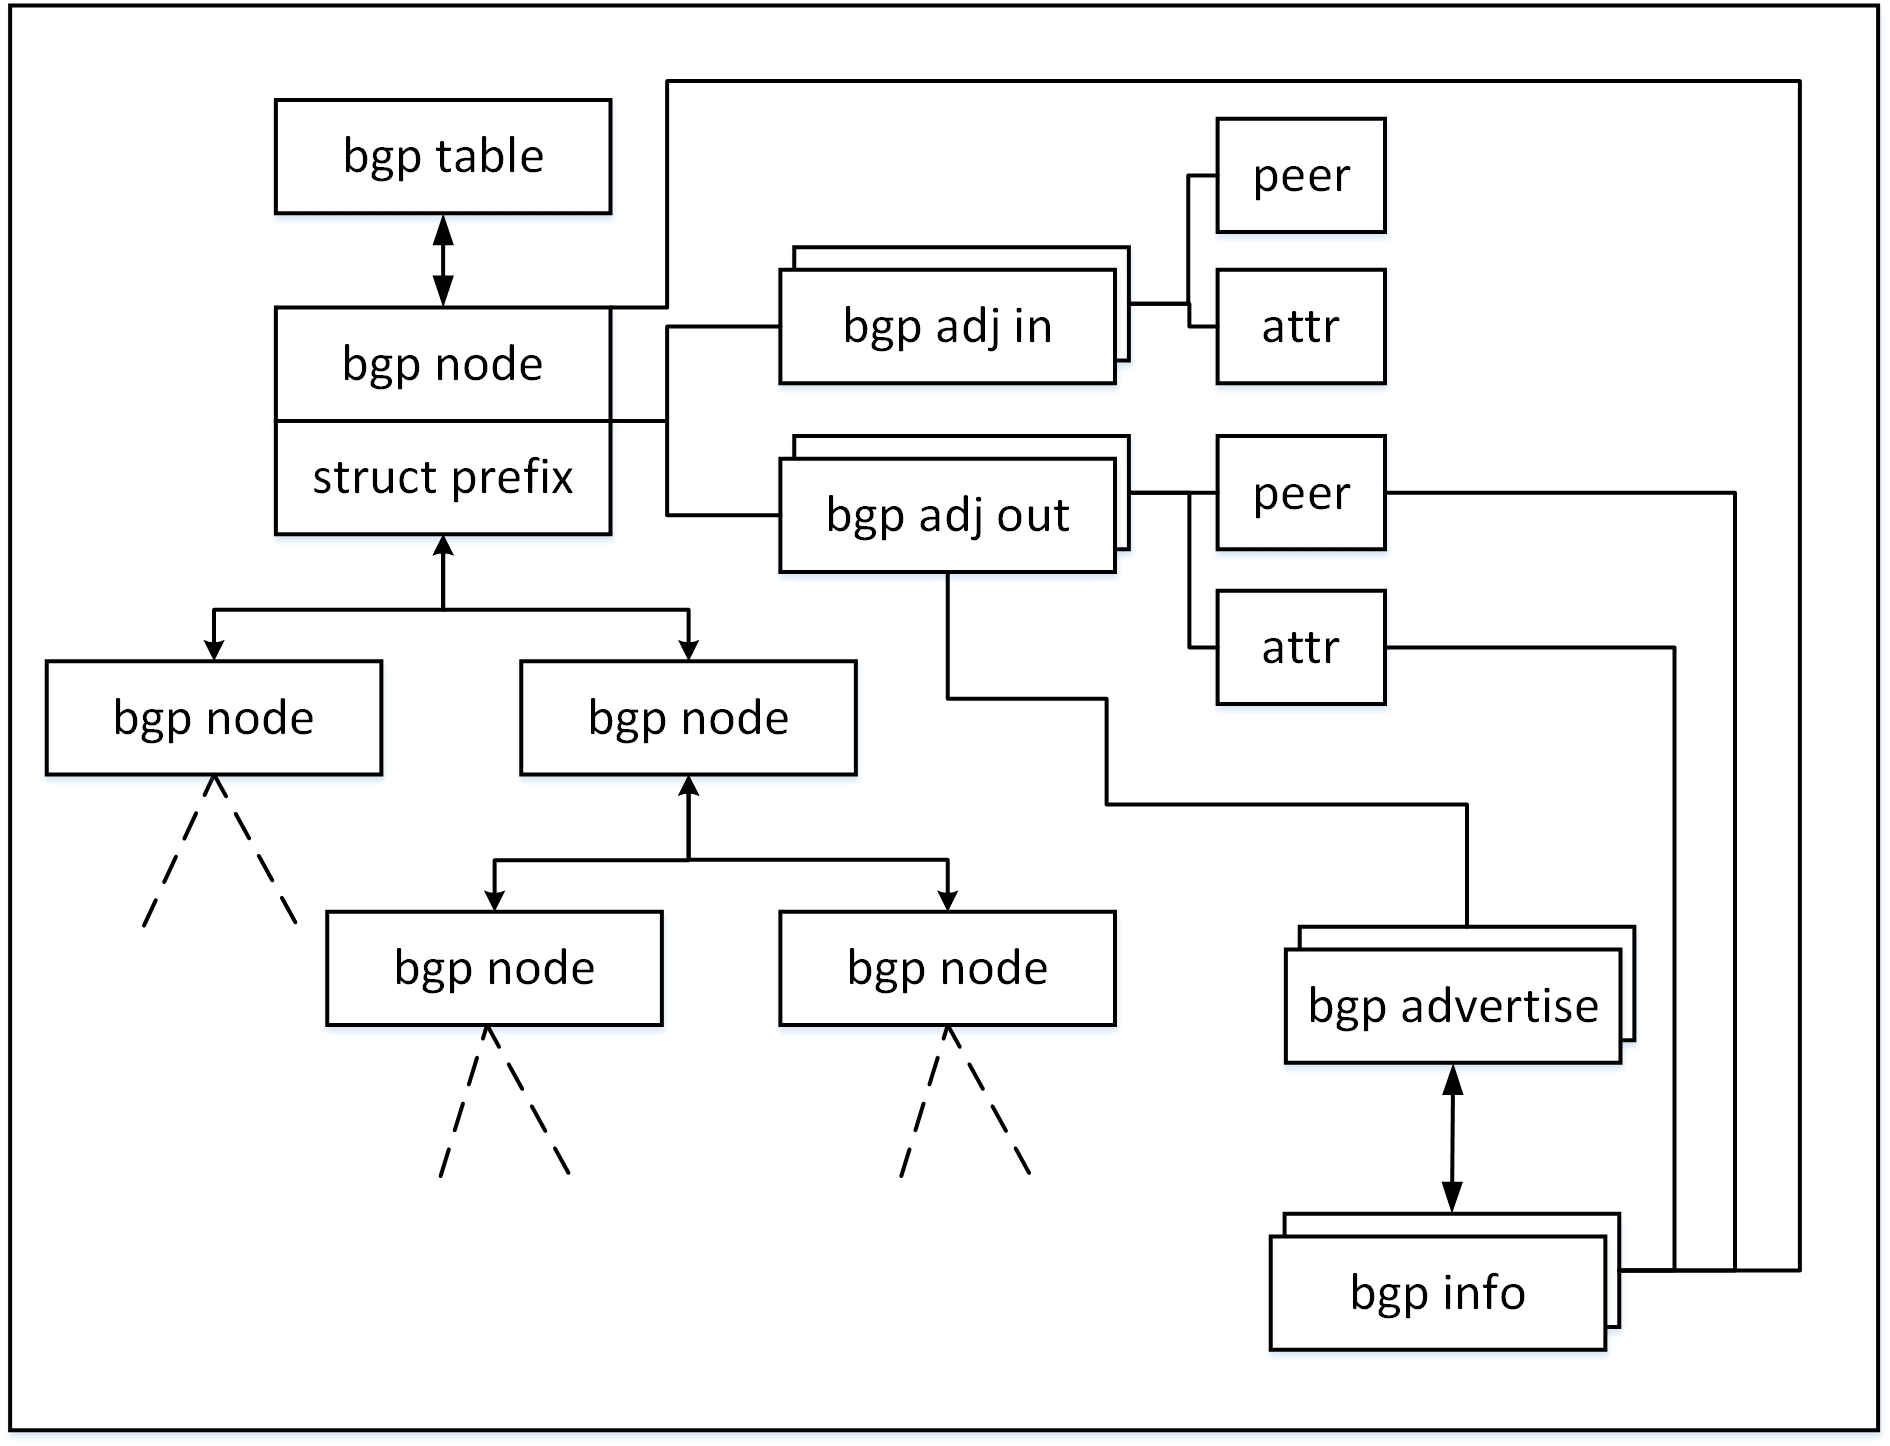
\includegraphics[width=0.75\textwidth]{storage}
  \caption{Quagga-bgpd:BGP路由表概括图\cite{jakma2014quagga}}
  \label{fig:storage}
\end{figure}

Quagga中路由表的存储使用radix二叉树\cite{quaggaThesis}存储结构,radix树是以二进制表示的键值作为树的节点,每个节点通过比较比特位来进行查找,radix二叉搜索树适合处理非常长的,可变长度的键值。每张Loc-RIB表存储在bgp\_table的结构体中,bgp\_table结构体有一个成员变量为bgp\_node类的结构体指针,该结构体指针是该Loc-RIB表radix树结构的根节点,所有路由表项的查找、删除等操作都从该根节点开始。bgp\_node结构体的实例代表的是某前缀所有的路由信息(每一条路由信息用bgp\_info结构体对应的实例表示),bgp\_node结构体中也存在指向bgp\_adj\_in和bgp\_adj\_out的指针。路由信息在bgp\_adj\_in和bgp\_adj\_out中的主要体现是通过他们的成员变量peer和attr。当BGP的某个邻居与之断开连接,则可以通过peer找到对应的prefix,清除bgp\_adj\_in且更新Loc-RIB。

当运行Quagga的虚拟路由器收到路有更新时,如果开启了Adj-RIBs-In存储设置,则会先根据前缀找到对应的bgp\_node,之后根据bgp\_node找到对应的adj\_rib\_in,对其进行更新。当BGP控制台需要输出某对等体的Adj-RIB-In表,则遍历所有的bgp\_node节点,根据bgp\_node找到每条前缀对应的adj\_rib\_in表,遍历该adj\_rib\_in表,如果某路由信息从该对等体收到的,则输出对应的路由信息。

针对某条路由信息bgp\_info向外进行路由宣告时,如果开启了Adj-RIBs-Out存储设置,则会先根据bgp\_info结构体中bgp\_node的指针,找到对应的bgp\_node,之后根据bgp\_node找到对应的adj\_rib\_out,对其进行更新。当BGP控制台需要输出某对等体的Adj-RIB-Out表,则遍历所有的bgp\_node节点,根据bgp\_node找到每条前缀对应的adj\_rib\_out表,遍历该adj\_rib\_out表,如果某路由信息从该对等体宣告出去,则输出对应的路由信息。

综合以上的文字解释,Quagga中实现BGP三张表的存储结构如图\ref{fig:storage}。
\subsection{路由更新流程}

\begin{figure}
  \centering
  % Requires \usepackage{graphicx}
  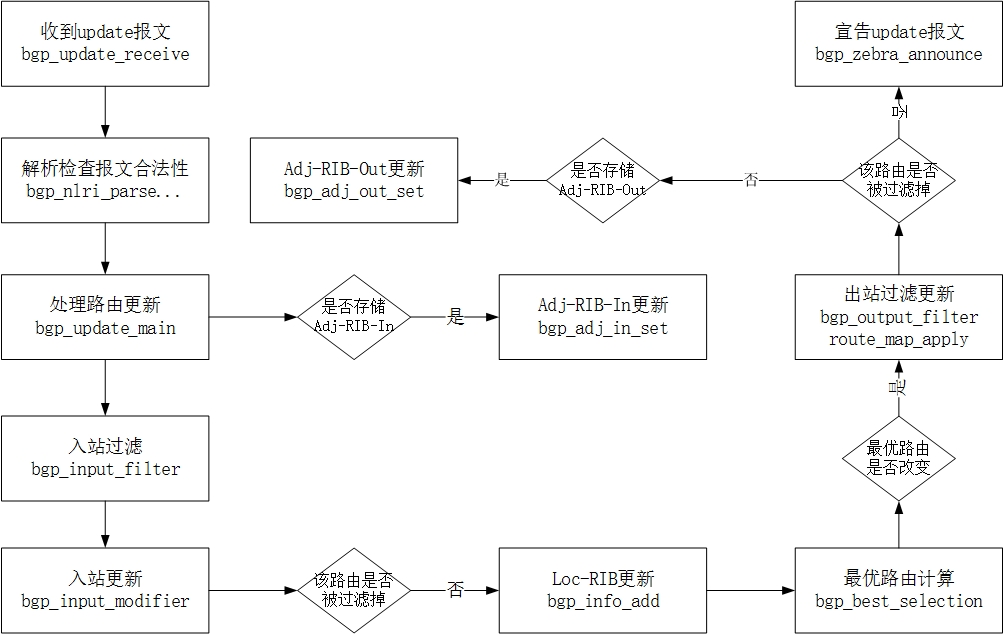
\includegraphics[width=0.8\textwidth]{route-update}
  \caption{Quagga-bgpd:BGP路由更新流程图}
  \label{fig:route-update}
\end{figure}



路由更新过程是虚拟路由器进行路由处理流程的主要部分,对应到Quagga中bgpd进程实现,路由更新的流程如图\ref{fig:route-update}:
\begin{itemize}
  \item 运行Quagga的虚拟路由器先通过bgp\_establish函数与对等体peer建立连接;
  \item 运行Quagga的虚拟路由器通过bgp\_read接收来自对等体的消息;
  \item 当收到BGP消息,通过检查头部的报文格式分析报文类型,如果是UPDATE报文,执行路由更新处理函数bgp\_update\_receive,进行UPDATE报文解析bgp\_nlri\_parse;
  \item 报文解析结束后,执行bgp\_update、bgp\_update\_main等函数进入路由更新消息的处理;
  \item 路由更新消息处理的过程中:如果需要存储Adj-RIBs-In表,进入bgp\_adj\_in\_set函数存储未经过滤的路由信息;之后执行入站过滤bgp\_input\_filter、入站更新bgp\_input\_modifier;如果更新路由没有被过滤掉,则将更新路由其通过info\_make函数生成bgp\_info信息;通过bgp\_info\_add函数将bgp\_info结构体的信息加入Loc\_RIB表中,然后将其通过bgp\_process函数将该bgp\_info路由信息的处理流程加入bgp\_process\_queue队列,该队列使用先进先出的策略;
  \item 当轮到该路由信息bgp\_info处理程序时,进入bgp\_process\_main函数,执行最优路由计算bgp\_best\_selection;
  \item 如果该前缀对应的最优路由发生改变,则执行bgp\_process\_announce\_selected函数,在该函数中有出站过滤更新bgp\_announce\_check和Adj-RIBs-Out更新bgp\_adj\_out\_set;
  \item 最终通过bgp\_zebra\_announce函数将BGP路由向外宣告,且将该最优路由信息注入到RIB表中。
\end{itemize}

\subsection{路由算法}


\begin{figure}
  \centering
  % Requires \usepackage{graphicx}
  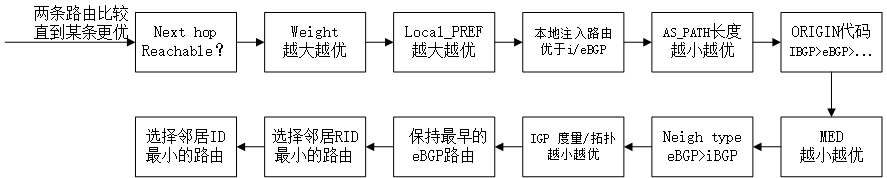
\includegraphics[width=0.9\textwidth]{route-cmp}
  \caption{Quagga-bgpd:BGP路由比较步骤}
  \label{fig:route-cmp}
\end{figure}

Quagga的bgpd进程中路由算法主要是在bgp\_best\_selection函数中实现的。针对前缀Prefix,在bgp\_table中找到该前缀对应的所有路由信息bgp\_node。路由信息的存储使用链表的数据结构,最新的路由会插在表头,所以bgp\_node存储的同一前缀的路由信息是按照更新时间由近及远进行存储。将该前缀对应的路由信息由近及远两两通过bgp\_info\_cmp进行比较,得到前缀的最优路由。两两比较选更优,比较步骤如图\ref{fig:route-cmp}。


\section{系统设计与实现}


本文提出的自治系统内的RSCP-iBGP系统的设计与实现主要涉及三大部分:自治系统内的边界路由器Route-Client路由器的设计与实现、自治系统内路由集中控制平台上Route-Server路由器的设计与实现、以及边界路由器Route-Client和路由集中控制平台Route-Server之间通信协议的设计与实现。


\subsection{边界路由器}

\begin{figure}
  \centering
  % Requires \usepackage{graphicx}
  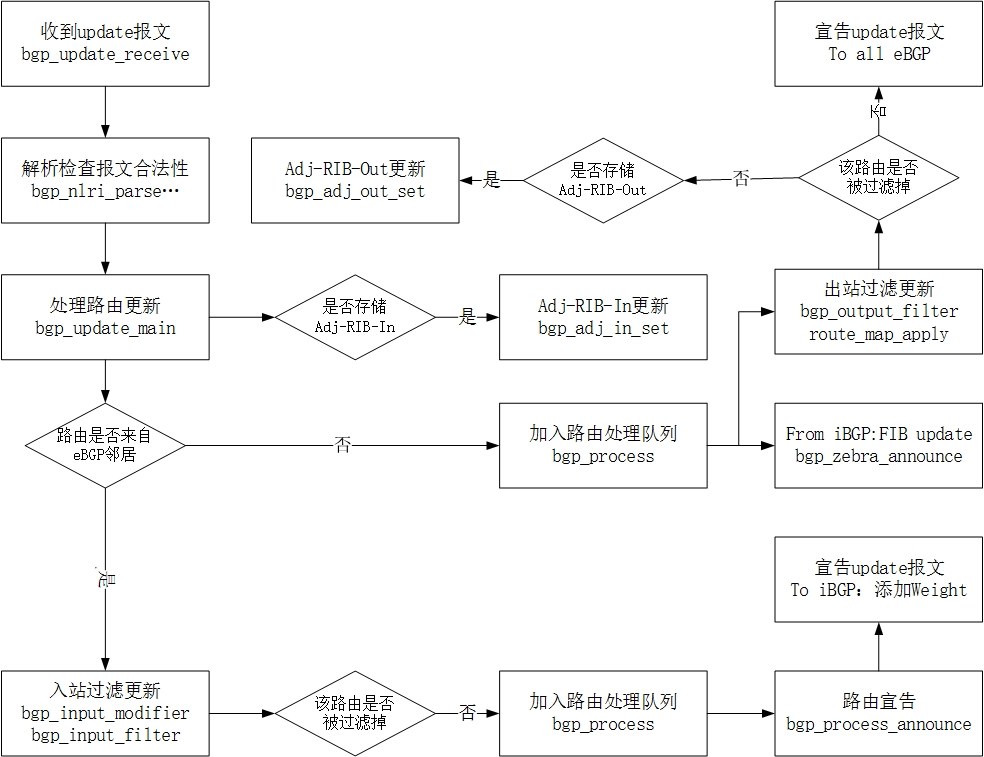
\includegraphics[width=0.9\textwidth]{rscp-route}
  \caption{RSCP-iBGP系统中边界路由器Route-Client:路由更新处理流程}
  \label{fig:rscp-route}
\end{figure}



边界路由器Route-Client收到集中平台Route-Server通过iBGP协议发来的最优路由,最优路由将会被提交到IP路由表中,相同前缀下拥有最低AD值的路由协议提交的最优路由最终会被放入IP路由表中,当路由器收到数据包时,根据IP路由表进行转发\cite{DianeTeare2016CCNP}。因为路由信息的存储和最优路由的计算均在路由控制平台上的Route-Server路由器完成,则边界路由器收到不同的路由信息(eBGP路由或者iBGP路由),需要执行不同的操作,具体的流程如图\ref{fig:rscp-route}。

当边界路由器Route-Client收到eBGP路由时,会先解析且检查该UPDATE报文的合法性,如果BGP配置文件中配置需要存储Adj-RIB-In,则将解析出来的路由信息存储到Adj-RIB-In表中。之后将该路由信息进行入站过滤和入站更新。如果该路由信息没有被eBGP的入站策略过滤掉,则将该路由加入路由处理队列等待处理。之后Route-Client会通过扩展的iBGP协议(将经过eBGP入站策略的Weight等路径属性和信息加入到UPDATE报文中),将该路由信息传输给集中平台上的Route-Server。


当边界路由器Route-Client收到iBGP路由时,会先解析且检查该UPDATE报文的合法性,如果BGP配置文件中配置需要存储Adj-RIB-In,则将解析出来的路由信息存储到Adj-RIB-In表中。该iBGP路由为路由控制平台为Route-Client计算出的最优路由,则将该路由加入路由处理队列等待处理。之后Route-Client需要将其更新到FIB表中,且将该路由信息经过出站过滤和出站更新。如果该路由信息没有被eBGP的出站策略过滤掉,则将其经过出站策略的最优路由宣告给所有的eBGP邻居。



\subsection{路由集中控制平台}

路由集中控制平台Route-Client主要对路由存储、路由计算进行了优化实现,其中RSCP-iBGP系统中的路由集中控制平台上运行的Quagga软件路由器BGP协议中路由宣告部分,也相对应需求进行了修改实现。

\subsubsection{增量路由存储}

集中控制平台上Route-Server路由器中的Loc-RIB路由存储不同于普通边界路由器的Loc-RIB路由存储。现有的自治系统内部如果有N台边界路由器,则Loc-RIB表需要存储N份。在RSCP-iBGP系统中,因为存在路由集中控制平台,则可以根据路径属性、路由比较算法等对路由信息进行增量存储。整个自治系统内的Loc-RIB均存储在路由集中控制平台Route-Server上,Route-Server上存储一张Public-Loc-RIB表,和N张iBGP邻居对应的Peer-Private-Loc-RIB表。

当收到一条UPDATE路由更新消息(Peer-info,Prefix-info, Attr-info),首先判断该路由更新是否存在于Public-Loc-RIB,如果不存在则加入Public-Loc-RIB。其次遍历每一张Peer[i]-Private-Loc-RIB表:如果表中有该Prefix且该路由信息不在Peer[i]-Private-Loc-RIB表中,则更新到对应的Peer[i]-Private-Loc-RIB;如果表中没有该Prefix,则当路由信息中的Weight属性值不为0,则仅将该更新路由更新到收到该路由信息的Route-Client边界路由器对应的Peer-Private-Loc-RIB中,同时将Public-Loc-RIB中该前缀之前的路由信息拷贝到Peer-Private-Loc-RIB,具体的实现见算法\ref{alg:incre_storage}。

\begin{algorithm}[!h]
    \caption{BGP\_INCREMENT\_STORAGE($Peer, Prefix, Attr$)}%算法标题
    \label{alg:incre_storage}
    \begin{algorithmic}[1]%一行一个标行号
        \REQUIRE
        $Peer, Prefix, Attr$
        \ENSURE
        $public\_rib, private\_ribs$
        \STATE $need\_add\_public\_rib \gets 1$
        \STATE $bgp\_info \gets make\_info(Peer, attr)$
        \IF{$(Prefix \in public\_rib) and (bgp\_info \in public\_rib[Prefix])$}
        \STATE $need\_add\_public\_rib \gets 0$
        \ENDIF
        \IF{$need\_add\_public\_rib = 1$}
        \STATE $bgp\_info\_add(bgp\_info, public\_rib[Prefix])$
        \ENDIF

        \FOR{each $Peer_i \in Established\_Peers$}
        \STATE $need\_add\_private\_rib \gets 0$

        \IF {$(Prefix \in Peer_i.private\_rib) and (bgp\_info \notin Peer_i.private\_rib[Prefix])$}
        \STATE $need\_add\_private\_rib \gets 1$
        \ENDIF
        \IF{$(Prefix \notin Peer_i.private\_rib) and (Attr.weight \ne 0) and (Peer = Peer_i)$}
        \STATE $need\_add\_private\_rib \gets 1$
        \FOR{each $(bgp\_info_i \in public\_rib[Prefix]) and (bgp\_info_i \ne bgp\_info)$}
        \STATE $bgp\_info\_add(bgp\_info_i, Peer_i.private\_rib[Prefix])$
        \ENDFOR
        \ENDIF

        \IF{$need\_add\_private\_rib = 1$}
        \STATE $bgp\_info\_add(bgp\_info, Peer_i.private\_rib[Prefix])$
        \ENDIF

        \ENDFOR
    \end{algorithmic}
\end{algorithm}


\subsubsection{复式路由计算}


在本文提出的RSCP-iBGP系统中的增量路由存储模块,路由计算结果与Weight路由属性相关的Prefix路由单独存储到Private\_Loc\_RIB,不受Weight路由属性影响的Prefix路由仅存储一份于Public\_Loc\_RIB。复式路由计算结合增量路由存储,与Weight相关的Peer的Prefix最优路由根据Peer的Private\_Loc\_RIB单独进行计算,其余的与Weight无关的Peer的Prefix最优路由通过Public\_Loc\_RIB进行计算。

当集中平台收到一条Prefix的路由信息时,需要计算出自治系统内所有边界路由器的该Prefix的最优路由。先通过Public\_Loc\_RIB表计算出所有Peer的最优路由,之后遍历所有对等体的Private\_Loc\_RIB,如果某个$Peer_i$的Private\_Loc\_RIB存储该Prefix的路由信息,则该$Peer_i$的Prefix最优路由更新为$Peer_i$的Private\_Loc\_RIB计算出的最优路由,具体实现见算法\ref{alg:multi_routing_calculation}。

\begin{algorithm}[htb]
    \caption{BGP\_Multi\_Routing\_Calculation($Peers, Prefix, public\_rib$)}%算法标题
    \label{alg:multi_routing_calculation}
    \begin{algorithmic}[1]%一行一个标行号
        \REQUIRE
        $Established\_Peers[1...j], Prefix, public\_rib$
        \ENSURE
        $Peer\_BestRoutes[1...j]$
        \STATE $Peer\_BestRoutes[1...j] \gets  bgp\_pub\_best\_selection(Prefix, public\_rib)$
        \FOR{each $Peer_i \in Established\_Peers[1...j]$}
        \IF {$(Prefix \in Peer_i.private\_rib)$}
        \STATE $Peer\_BestRoutes[i] \gets  bgp\_pri\_best\_selection(Prefix, Peer_i.private\_rib)$
        \ENDIF
        \ENDFOR
        \RETURN $Peer\_BestRoutes[1...j]$
    \end{algorithmic}
\end{algorithm}

通过路由集中控制平台Route-Server中存储的Public\_Loc\_RIB表,计算出与Weight无关的所有Peer针对Prefix的最优路由。使用Public\_Loc\_RIB计算所有边界路由器最优路由的过程,主要分为两大部分:
\begin{itemize}
  \item 各边界路由器的衡量标准相同,依次执行删除Prefix对应的路由集合中非最高本地优先级、非最短As-path、相同AS非最低MED值等3个操作,在每个操作之后判断该Prefix对应的路由集合中是否仅剩一条路由,如果仅剩一条路由,则为所有边界路由器的该Prefix的最优路由,具体实现见算法\ref{alg:public_selection_one};
  \item 因为边界路由器之间的IGPcost各有不同,所以如果在各边界路由器衡量标准相同的筛选条件下没有计算出最优路由,则之后为自治系统内的每台边界路由器计算最优路由需要单独进行计算,基于Prefix对应的路由集合依次执行删除非最短IGPcost的路由、非最早eBGP路由、非最小的接收该路由的eBGP邻居route-id(存储在路由集中平台)、非最小的接收该路由的eBGP邻居IP地址(存储在路由集中平台)等操作,在每个操作之后判断该Prefix对应的路由集合中是否仅剩一条路由,如果仅剩一条路由,则为该边界路由器对应的该Prefix的最优路由,具体实现见算法\ref{alg:public selection_two}。
\end{itemize}


与Weight相关的Peer的Prefix最优路由,需要根据Peer的Private\_Loc\_RIB表中的Prefix的全部路由进行单独计算,通过将Peer的Private\_Loc\_RIB表中的Prefix的全部路由放入路由集合,依次删除路由集合中的非最大Weight值、非最高本地优先级、非最短As-path、相同AS非最低MED值、非最短IGPcost的路由、非最早eBGP路由、非最小的接收该路由的eBGP邻居route-id(存储在路由集中平台)、非最小的接收该路由的eBGP邻居IP地址(存储在路由集中平台)等操作。在每个操作之后判断该Prefix对应的路由集合中是否仅剩一条路由,如果仅剩一条路由,则为该边界路由器对应的该Prefix的最优路由。

\begin{algorithm}[!h]
    \caption{bgp\_pub\_best\_selection($Prefix, public\_rib, Established\_Peers$)}
    \label{alg:public_selection_one}
    \begin{algorithmic}[1]%一行一个标行号
        \REQUIRE
        $Prefix, public\_rib, Established\_Peers[1...j]$
        \ENSURE
        $Peer\_BestRoutes[1...j]$
        \STATE $Public\_BestRoute \gets NULL$
        \STATE $public\_rib\_t \gets public\_rib$
        \STATE $public\_rib\_t \gets delete\_nonMaxLocPref(public\_rib\_t)$
        \IF {$public\_rib\_t.size = 1$}
        \STATE $Public\_BestRoute  \gets public\_rib\_t[0]$
        \ENDIF

        \STATE $public\_rib\_t \gets delete\_nonMinAsPathLength(public\_rib\_t)$
        \IF {$public\_rib\_t.size = 1$}
        \STATE $Public\_BestRoute  \gets public\_rib\_t[0]$
        \ENDIF

        \STATE $public\_rib\_t \gets delete\_nonMinMedSameAs(public\_rib\_t)$
        \IF {$public\_rib\_t.size = 1$}
        \STATE $Public\_BestRoute  \gets public\_rib\_t[0]$
        \ENDIF

        \IF {$Peer\_BestRoutes \ne NULL$}
        \FOR{each $Peer\_BestRoutes[i] \in Peer\_BestRoutes[1...j]$}
        \STATE $Peer\_BestRoutes[i] \gets Public\_BestRoute $
        \ENDFOR
        \STATE \textbf{return} $Peer\_BestRoutes[1...j]$
        \ENDIF

        \FOR{each $Peer_i \in Established\_Peers[1...j]$}
        \STATE $Peer\_BestRoutes[i] \gets get\_specialBestRoute\_fromPublicRib(peer_i,public\_rib\_t)$
        \ENDFOR
        \STATE \textbf{return} $Peer\_BestRoutes[1...j]$
    \end{algorithmic}
\end{algorithm}





\subsubsection{路由宣告}
当自治系统内的路由集中控制平台Route-Server路由器收到自治系统内的边界路由器Route-Client发来的iBGP路由,对该iBGP路由信息进行解析(包括从UPDATE报文中解析Weight路径属性),Router-Server会根据存储的路由表项计算出该路由前缀的针对自治系统内所有边界路由器的最优路由,最后将对应的最优路由宣告给对应的边界路由器(如果边界路由器Route-Client-i的最优路由是该边界路由器自身Route-Client-i收到的,next-hop设置为对应的直连eBGP邻居;如果边界路由器Route-Client-i的最优路由是其他边界路由器Route-Client-j从eBGP邻居收到的,next-hop设置为Route-Client-j的与Route-Client-i一个网段的地址)。

在路由宣告的过程中,Route-Server上运行的软件路由器会检测宣告路由的合法性,因为Quagga版本中判断路由器是否为路由反射器的标准为该路由信息是否从iBGP邻居接收并宣告给iBGP邻居,所以在Route-Server上运行的软件路由器代码需要在接收路由后或者宣告路由前,对路由反射器的检测代码进行修改。

传统的路由信息传输到路由器之后,路由器会检测其Next-hop值是否可达,则一般会通过在BGP的配置文件中给iBGP邻居设置Next-hop-self属性,保证Next-hop可达性。在本文提出的RSCP-iBGP系统中,需要在集中控制平台上进行最优路由的计算,并将最后的计算结果通过iBGP协议传输给边界路由器Route-Client,则需要将eBGP邻居的Next-hop值传输到集中平台,则不设置Next-hop-self属性,Route-Client边界路由器会将eBGP邻居的Next-hop值传到集中平台,且在集中平台上暂时不做可达性检测。未来可将Route-Client的eBGP可达邻居信息进行实时管理更新,基于集中平台上管理的自治系统内部的Route-Client的eBGP可达邻居信息,可在集中平台Route-Server上判断路由从eBGP邻居过来的Next-hop的可达性,从而确保路由信息的有效性。

\begin{algorithm}[!h]
    \caption{get\_specialBestRoute\_fromPublicRib($peer,public\_rib$)}
    \label{alg:public selection_two}
    \begin{algorithmic}[1]%一行一个标行号
         \REQUIRE
        $peer,public\_rib$
        \ENSURE
        $Peer\_BestRoute$
        \STATE $public\_rib\_t \gets public\_rib$
        \STATE $public\_rib\_t \gets delete\_nonMinIGPcost(peer, public\_rib\_t)$
        \IF {$public\_rib\_t.size = 1$}
        \STATE \textbf{return} $public\_rib\_t[0]$
        \ENDIF
        \STATE $public\_rib\_t \gets delete\_nonEarliestRoute(peer, public\_rib\_t)$
        \IF {$public\_rib\_t.size = 1$}
        \STATE \textbf{return} $public\_rib\_t[0]$
        \ENDIF
        \STATE $public\_rib\_t \gets delete\_nonMinEbgpPeer\_Route-id(peer, public\_rib\_t)$
        \IF {$public\_rib\_t.size = 1$}
        \STATE \textbf{return} $public\_rib\_t[0]$
        \ENDIF
        \STATE $public\_rib\_t \gets delete\_nonMinEbgpPeer\_IPAddr(peer, public\_rib\_t)$
        \IF {$public\_rib\_t.size = 1$}
        \STATE \textbf{return} $public\_rib\_t[0]$
        \ENDIF
        \STATE \textbf{return} $public\_rib\_t[0]$
    \end{algorithmic}
\end{algorithm}


\subsection{通信接口}
通信接口通过扩展的iBGP协议进行实现,边界路由器Route-Client需要发送携带Weight路径属性的UPDATE报文信息到集中平台Route-Server,且Route-Server收到扩展iBGP协议发来的携带Weight路径属性的UPDATE报文需要能够进行正常识别和解析。

边界路由器上运行的BGP协议需要在给iBGP邻居发送UPDATE报文的时候携带Weight路径属性,所以在边界路由器上运行的软件路由器Quagga中,需要修改UPDATE报文的Path Attributes部分,增加传输Weight路径属性。在Quagga中的BGP协议代码实现UPDATE报文中,Path Attributes的组包实现函数为bgp\_packet\_attribute(bgpd\_attr.c文件中),在其他属性添加结束后,在字节流后添加Path Attribute的三元组,具体的实现见算法\ref{alg:add_weight}。传输Weight属性的三元组中,Flag=0x40和Type Code=0x1f,Length=0x02,Value值长度为2个字节。如果传输的Weight值为150,则对应的传输Weight的Path  Attribute为0x401f020096。

\begin{algorithm}[!h]
    \caption{BGP\_PACKET\_ATTRIBUTE($peer,attr,stream...$)}%算法标题
    \label{alg:add_weight}
    \begin{algorithmic}[1]%一行一个标行号
        \STATE $stream \gets Path\_Attributes\_Except\_Weight\_Info$
        \IF{$peer->sort = BGP\_PEER\_IBGP$}
        \STATE $stream \gets stream+BGP\_ATTR\_FLAG\_TRANS$
        \STATE $stream \gets stream+BGP\_ATTR\_WEIGHT\_TYPE\_CODE$
        \STATE $stream \gets stream+BGP\_ATTR\_WEIGHT\_LENGTH$
        \STATE $stream \gets stream+BGP\_ATTR\_WEIGHT\_VALUE$
        \ENDIF
    \end{algorithmic}
\end{algorithm}


集中平台上Route-Server收到携带Weight路径属性值的UPDATE报文后,需要对其进行正确的解析。Quagga中的BGP协议代码实现Path Attributes解析的函数为bgp\_attr\_parse(bgpd\_attr.c文件中),根据Type Code执行不同的Path Attribute解析函数,Weight属性的解析函数需要检查Length是否为2。如果不为2,需要执行bgp\_notify\_send函数,回复对等体NOTIFICATION报错(Path Attribute长度错误)。



\section{本章小结}
本章对RSCP-iBGP系统的实现平台Quagga进行了详细的介绍,了解虚拟路由器Quagga的BGP路由实现之后,针对RSCP-iBGP系统的需求,具体描述了RSCP-iBGP系统中边界路由器、集中控制平台,通信协议的设计与实现。

\chapter{仿真实验与一致性测试}
\label{cha:evaluate}


\section{本章引言}
本章主要对RSCP-iBGP系统的功能进行了测试评价、对新系统下的两种路由器Route-Server和Route-Client的功能进行了一致性测试。通过设计合理的网络拓扑,验证RSCP-iBGP系统实现了路由存储和路由计算的集中优化、在路由计算的过程中基于全部路由且不存在因为MED不可比引起路由震荡等功能。本章节通过TTCN-3测试例对RSCP-iBGP新系统中的Route-Server路由器和Route-Client路由器进行一致性测试,很好地验证了RSCP-iBGP系统功能实现与设计的一致性。

\section{RSCP-iBGP系统功能验证实验}

\subsection{路由存储集中优化}


\begin{figure}
  \centering
  % Requires \usepackage{graphicx}
  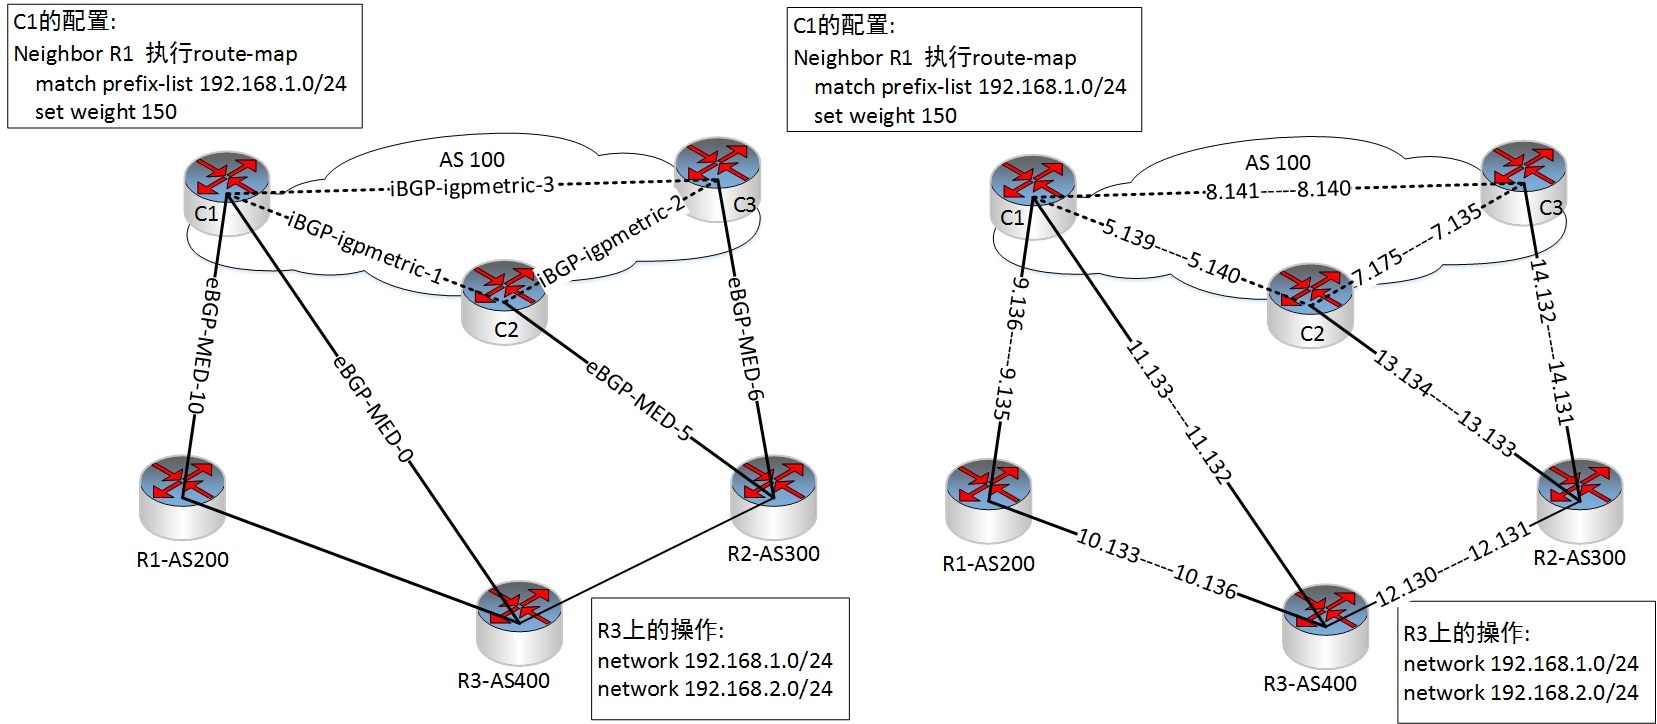
\includegraphics[width=\textwidth]{loc-rib-example-fm}
  \caption{自治系统内iBGP全连接的网络拓扑图}
  \label{fig:loc-rib-example-fm}
\end{figure}

在本文提出的RSCP-iBGP系统中,自治系统内的Loc-RIB路由信息均存储在集中平台的Route-Server路由器上,路由存储集中优化是否实现正确,通过运行图\ref{fig:loc-rib-example-ip}中的拓扑进行检测验证,与之对应的自治系统内全连接的拓扑结构如图\ref{fig:loc-rib-example-fm}。

使用虚拟机搭建图\ref{fig:loc-rib-example-fm}的网络拓扑,安装了Linux系统的虚拟机运行软件路由器Quagga来模拟真实的路由器。在图\ref{fig:loc-rib-example-fm}中自治系统号为100的自治系统内部的边界路由器之间通过iBGP协议两两连接。分别在R1、R2、C1上使用Route-map过滤更新策略,来配置BGP策略,使得从R1宣告给C1的路由MED值=10,从R2宣告给C2的路由MED=5,从R2宣告给C3的路由MED=6,从R1收到的Prefix为192.168.1.0/24的路由信息经过C1的入站策略后该路由的Weight值改为150,通过iBGP协议传输的iBGP路由信息Local Preference默认为100(路由比较过程中如果LocPrf值未设置,默认为100)。则当R3向外宣告192.168.1.0/24和192.168.2.0/24时,自治系统号为100的自治系统内的边界路由器的Loc-RIB表格分别为表\ref{fig:c1-table}、表\ref{fig:c2-table}、表\ref{fig:c3-table}:

%\begin{table}[]
%\centering
%\caption{自治系统内全连接拓扑下C1的Loc-RIB表项}
%\label{tab:cl-fm}
%\begin{tabular}{|c|c|c|c|c|c|c|}
%\hline
%Network     & \begin{tabular}[c]{@{}c@{}}Origin\\ code\end{tabular} & Next Hop          & Metirc & LocPrf & Weight & Aspaths   \\ \hline
%192.168.1.0 & i                                                   & 192.168.5.140-C2  & 5      & 100    & 0      & 300 400 i \\ \hline
%            &                                                    & 192.168.9.135-R1 & 10      &        & 150      & 200 400 i \\ \hline
%            &                                                      & 192.168.11.132-R3  & 0     &     & 0      & 400 i \\ \hline
%192.168.2.0 &                                                      & 192.168.9.135-R1 & 10      &        & 0      & 200 400 i \\ \hline
%            &                                                     & 192.168.11.132-C3  & 0      &     & 0      & 400 i     \\ \hline
%\end{tabular}
%\end{table}

\begin{figure}
  \centering
  % Requires \usepackage{graphicx}
  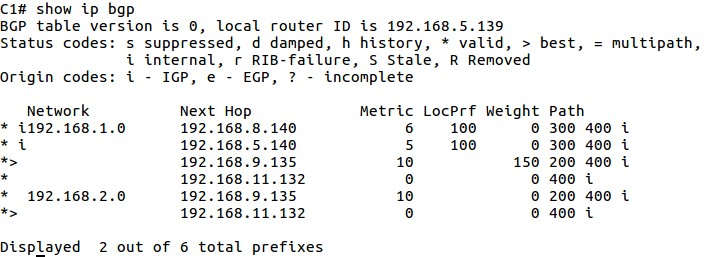
\includegraphics[width=0.8\textwidth]{c1-table}
  \caption{自治系统内全连接拓扑下C1的Loc-RIB表项}
  \label{fig:c1-table}
\end{figure}


\begin{figure}
  \centering
  % Requires \usepackage{graphicx}
  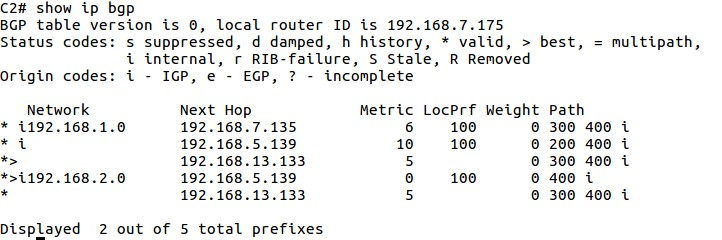
\includegraphics[width=0.8\textwidth]{c2-table}
  \caption{自治系统内全连接拓扑下C2的Loc-RIB表项}
  \label{fig:c2-table}
\end{figure}

\begin{figure}
  \centering
  % Requires \usepackage{graphicx}
  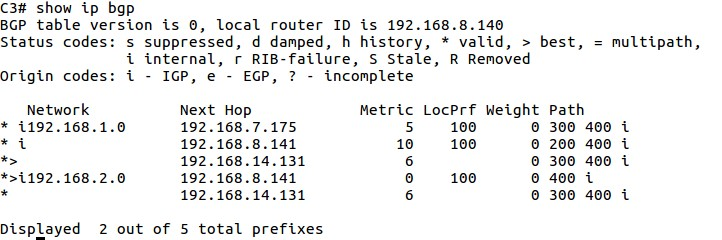
\includegraphics[width=0.8\textwidth]{c3-table}
  \caption{自治系统内全连接拓扑下C3的Loc-RIB表项}
  \label{fig:c3-table}
\end{figure}

%\begin{table}[]
%\centering
%\caption{自治系统内全连接拓扑下C2的Loc-RIB表项}
%\label{tab:c2-fm}
%\begin{tabular}{|c|c|c|c|c|c|c|}
%\hline
%Network     & \begin{tabular}[c]{@{}c@{}}Origin\\ code\end{tabular} & Next Hop          & Metirc & LocPrf & Weight & Aspaths   \\ \hline
%192.168.1.0 &                                                       & 192.168.13.133-R2  & 5      &        & 0      & 300 400 i \\ \hline
%            & i                                                     & 192.168.5.139-C1 & 10     & 100    & 0      & 200 400 i \\ \hline
%192.168.2.0 &                                                       & 192.168.13.133-R2 & 5      &        & 0      & 300 400 i \\ \hline
%            & i                                                     & 192.168.5.139-C1  & 0      & 100    & 0      & 400 i     \\ \hline
%\end{tabular}
%\end{table}


%\begin{table}[]
%\centering
%\caption{自治系统内全连接拓扑下C3的Loc-RIB表项}
%\label{tab:c3-fm}
%\begin{tabular}{|c|c|c|c|c|c|c|}
%\hline
%Network     & \begin{tabular}[c]{@{}c@{}}Origin\\ code\end{tabular} & Next Hop          & Metirc & LocPrf & Weight & Aspaths   \\ \hline
%192.168.1.0 & i                                                     & 192.168.7.175-C2  & 5      & 100    & 0      & 300 400 i \\ \hline
%            &                                                       & 192.168.14.131-R2 & 6      &        & 0      & 300 400 i \\ \hline
%            & i                                                     & 192.168.8.141-C1  & 10     & 100    & 0      & 200 400 i \\ \hline
%192.168.2.0 &                                                       & 192.168.14.131-R2 & 6      &        & 0      & 300 400 i \\ \hline
%            & i                                                     & 192.168.8.141-C1  & 0      & 100    & 0      & 400 i     \\ \hline
%\end{tabular}
%\end{table}

\begin{figure}
  \centering
  % Requires \usepackage{graphicx}
  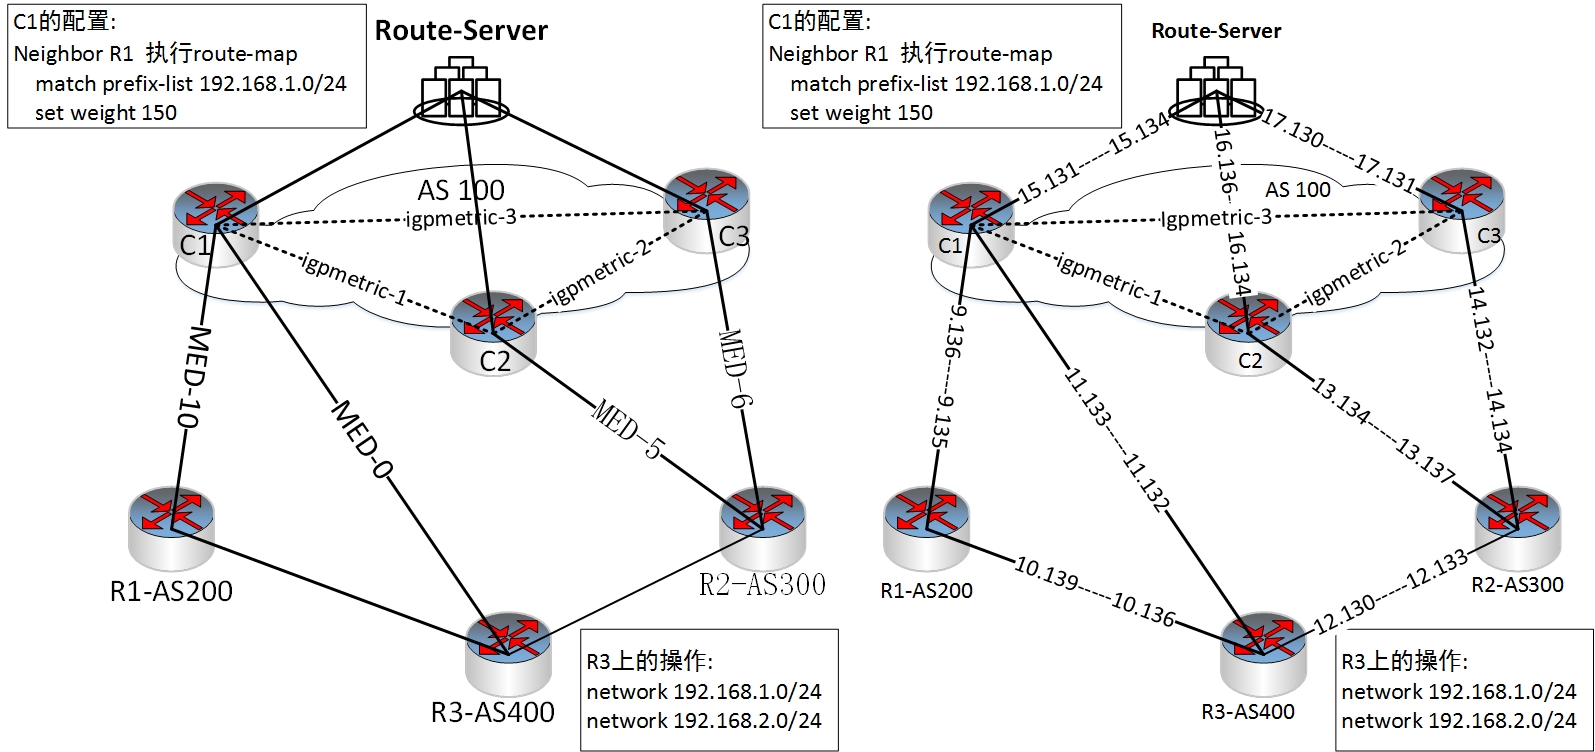
\includegraphics[width=\textwidth]{loc-rib-example-ip}
  \caption{自治系统内RSCP-iBGP系统的网络拓扑图}
  \label{fig:loc-rib-example-ip}
\end{figure}


使用虚拟机搭建图\ref{fig:loc-rib-example-ip}的网络拓扑,自治系统号为100的自治系统外的边界路由器通过安装了Linux系统的虚拟机运行软件路由器Quagga来,自治系统号为100的自治系统内部部署RSCP-iBGP系统,自治系统号为100的自治系统内的边界路由器通过安装了Linux系统的虚拟机运行修改后的软件路由器Quagga-Route-Client来模拟,自治系统号为100的自治系统内的Route-Server路由器通过安装了Linux系统的虚拟机,虚拟机运行修改后的软件路由器Quagga-Route-Server来模拟。仍需在R1、R2、C1上使用Route-map过滤更新策略来配置BGP策略,使得从R1宣告给C1的路由MED值=10,从R2宣告给C2的路由MED=5,从R2宣告给C3的路由MED=6,从R1收到的Prefix192.168.1.0/24的路由信息经过C1的入站策略后该路由的Weight值改为150,通过iBGP协议传输的iBGP路由信息Local Preference默认为100。则当R3向外宣告192.168.1.0/24和192.168.2.0/24时,自治系统号为100的自治系统内Route-Server路由器上存储的Public-Loc-RIB见图\ref{fig:public-table}。 192.168.1.0/24和192.168.2.0/24前缀的最优路由与Weight相关的仅有C1边界路由器,则Route-Server仅存储了针对C1的Private-Loc-RIB,见表\ref{fig:private-table}。


\begin{figure}
  \centering
  % Requires \usepackage{graphicx}
  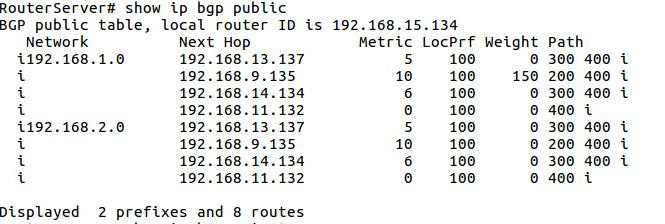
\includegraphics[width=0.8\textwidth]{public-table}
  \caption{Route-Server路由器中的Public-Loc-RIB表项}
  \label{fig:public-table}
\end{figure}

%\begin{table}[]
%\centering
%\caption{Route-Server路由器中的Public-Loc-RIB表项}
%\label{tab:pub}
%\begin{tabular}{|c|c|l|c|c|c|c|}
%\hline
%Network     & \begin{tabular}[c]{@{}c@{}}Received\\ iBGP-Peer\end{tabular} & Next Hop & Metric & LocPrf & Weight & Aspaths   \\ \hline
%192.168.1.0 & C1                                                           & R3       & 0      & 100    &  /    & 400,i     \\ \hline
%192.168.1.0 & C1                                                           & R1       & 10     & 100    & /    & 200,400,i \\ \hline
%192.168.1.0 & C2                                                           & R2       & 5      & 100    &  /     & 300,400,i \\ \hline
%192.168.1.0 & C3                                                           & R2       & 6      & 100    &   /     & 300,400,i \\ \hline
%192.168.2.0 & C1                                                           & R3       & 0      & 100    &  /      & 400,i     \\ \hline
%192.168.2.0 & C1                                                           & R1       & 10     & 100    &  /      & 200,400,i \\ \hline
%192.168.2.0 & C2                                                           & R2       & 5      & 100    &  /      & 300,400,i \\ \hline
%192.168.2.0 & C3                                                           & R2       & 6      & 100    &  /      & 300,400,i \\ \hline
%\end{tabular}
%\end{table}



%\begin{table}[]
%\centering
%\caption{Route-Server路由器中的针对C1的Private-Loc-RIB表项}
%\label{tab:pri}
%\begin{tabular}{|c|c|l|c|c|c|c|}
%\hline
%Network     & \begin{tabular}[c]{@{}c@{}}Received\\ iBGP-Peer\end{tabular} & Next Hop & Metric & LocPrf & Weight & Aspaths   \\ \hline
%192.168.1.0 & C1                                                           & R3       & 0      & 100    &      & 400,i     \\ \hline
%192.168.1.0 & C1                                                           & R1       & 10     & 100    & 150    & 200,400,i \\ \hline
%192.168.1.0 & C2                                                           & R2       & 5      & 100    &       & 300,400,i \\ \hline
%192.168.1.0 & C3                                                           & R2       & 6      & 100    &        & 300,400,i \\ \hline
%\end{tabular}
%\end{table}


传统的Loc-RIB路由信息,存储于自治系统内部的边界路由器上。假设自治系统内有N台路由器,外部有M条路由传到该自治系统,则每台路由器存储约M条Loc-RIB路由表项,自治系统内总共存储约N*M条路由信息。在图\ref{fig:loc-rib-example-fm}的拓扑条件下,自治系统号为100的自治系统共存储了约N*M(N=3)条路由。而本文提出的RSCP-iBGP系统中只需存储一份M条表项的Public-Loc-RIB信息和若干份与Weight值相关的m条表项的前缀路由信息,则自治系统共存储M+m条路由信息,因为m远小于M,则自治系统共存储了约M条路由表项。在图\ref{fig:loc-rib-example-ip}的拓扑条件下,自治系统号为100的自治系统共存储了约M+m(m远小于M)条路由。相比于传统的分布式路由存储方式,本文提出的RSCP-iBGP系统中的增量路由存储将需要路由表项的总数下降了一个数量级(N份下降到1份),对路由存储进行了优化。

\begin{figure}
  \centering
  % Requires \usepackage{graphicx}
  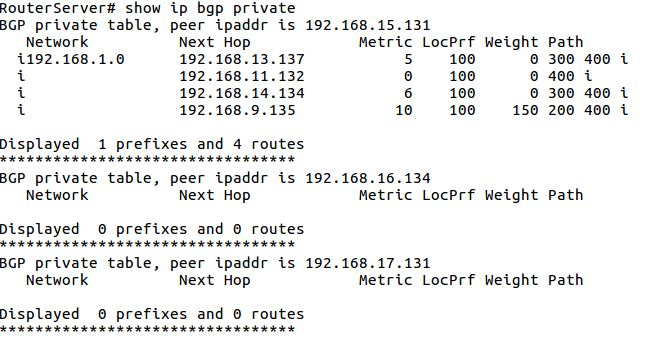
\includegraphics[width=0.8\textwidth]{private-table}
  \caption{Route-Server路由器中的针对Peer的Private-Loc-RIB表项}
  \label{fig:private-table}
\end{figure}

\subsection{路由计算集中优化}

在图\ref{fig:loc-rib-example-fm}的拓扑条件下,路由策略配置使得从R1宣告给C1的路由MED值=10,从R2宣告给C2的路由MED=5,从R2宣告给C3的路由MED=6,从R1收到的Prefix192.168.1.0/24的路由信息经过C1的入站策略后该路由的Weight值改为150,通过iBGP协议传输的iBGP路由信息Local Preference默认为100(路由比较过程中如果LocPrf值未设置,默认为100)。则当R3向外宣告192.168.1.0/24和192.168.2.0/24前缀时,C1、C2、C3分别根据自己收到的路由和路由策略,分别计算最优路由。

C1针对192.168.1.0/24前缀计算出的最优路由是C1-R1-R3, C1针对192.168.2.0/24前缀计算出的最优路由是C1-R3;C2针对192.168.1.0/24前缀计算出的最优路由是C2-R2-R3, C2针对192.168.2.0/24前缀计算出的最优路由是C2-C1-R3;C3针对192.168.1.0/24前缀计算出的最优路由是C3-R2-R3, C3针对192.168.2.0/24前缀计算出的最优路由是C3-C1-R3,每收到一条新路由,均会进行一次路由计算,则总共计算了6+5+5=16次。在全连接的拓扑图\ref{fig:loc-rib-example-fm}中,R3宣告了2个前缀,共8条路由传入自治系统,最后路由收敛后最优路由计算了16次。若自治系统内有N台边界路由器,当一条更新路由传到自治系统时,每台边界路由器均需进行路由更新流程,如果最优路由发生变化则需要进行再次宣告,进入路由收敛过程,在这个过程中路由计算最少N次,最多N\verb+*+(N-1)/2次。


在图\ref{fig:loc-rib-example-ip}的拓扑条件下,路由策略配置使得从R1宣告给C1的路由MED值=10,从R2宣告给C2的路由MED=5,从R2宣告给C3的路由MED=6,从R1收到的Prefix192.168.1.0/24的路由信息经过C1的入站策略后该路由的Weight值改为150,通过iBGP协议传输的iBGP路由信息Local Preference默认为100(路由比较过程中如果LocPrf值未设置,默认为100)。则当R3向外宣告192.168.1.0/24和192.168.2.0/24前缀时,C1、C2、C3分别根据自己收到的路由传输到集中平台Route-Server路由器,Route-Server根据全部的路由信息为每一台边界路由器计算最优路由。

针对192.168.1.0/24前缀,Route-Server共收到4条路由,最后一次收到的路由与weight有关,则前3次收到路由分别各经过1次计算得到C1、C2、C3的最优路由,最后一次通过Public-Loc-RIB计算1次得到C2和C3的最优路由,再通过针对C1的Private-Loc-RIB计算1次得到C1的最优出口,则传入集中平台4条路由,共计算了5次最优路由。针对192.168.2.0/24前缀,Route-Server收到了4条路由,每收到一条路由均仅需计算一次即可得到C1、C2、C3的最优路由,因为192.168.2.0/24最优路由的决定性条件是Aspath长度,这属于所有边界路由器相同的可比路由属性,且其相关路由与Weight值不相关。最终共8条路由传入自治系统,最后最优路由共计算了9次,相比全连接的16次,减少了不少计算次数。因为不存在路由收敛,所以当一条新路由传输到自治系统,RSCP-iBGP系统路由计算最少1次,最多N次。相比有路由收敛的传统分布式路由,本文提出的RSCP-iBGP将当新路由到达自治系统时,自治系统内的路由计算次数平均优化了一个数量级。

\subsection{基于全部路由且无MED值引起的路由震荡}


\begin{figure}
  \centering
  % Requires \usepackage{graphicx}
  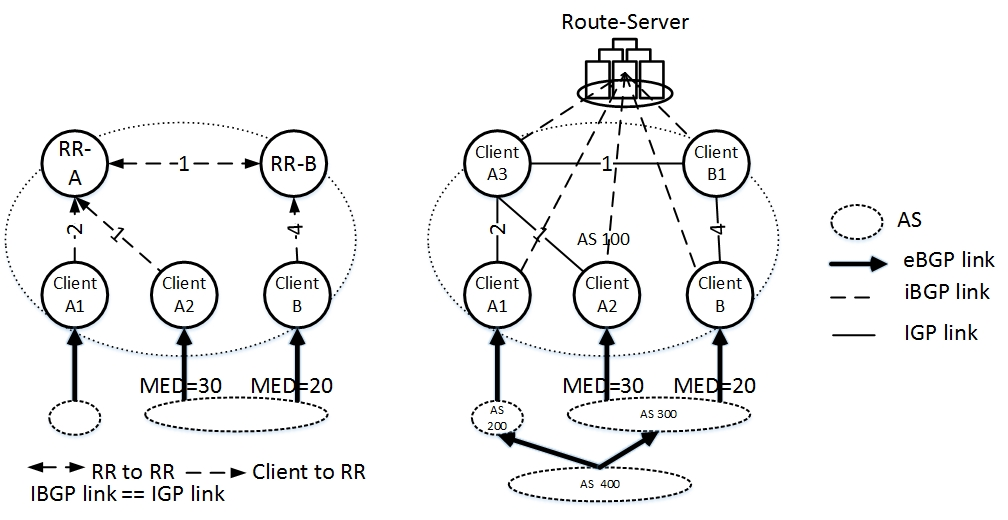
\includegraphics[width=0.75\textwidth]{rscp-fixmed}
  \caption{RSCP-iBGP系统下解决RR引起的MED路由震荡的实验拓扑}
  \label{fig:rscp-fixmed}
\end{figure}


本文提出的RSCP-iBGP系统中的复式路由计算,基于全部的路由进行计算。路由计算的过程采用集合排除法,当自治系统相同的时候,从Prefix的路由集合中删除MED值更大的路由,保证路由更新到达顺序不一致的情况下,最终当基于全部路由进行计算的时候,得到的最优路由是确定的。以RR路由反射引起的MED路由震荡为例,如图\ref{fig:rscp-fixmed}。

通过虚拟机搭建图\ref{fig:rscp-fixmed}中右侧拓扑的网络环境,AS400的边界路由器向外宣告192.168.1.0/24前缀。通过查看Route-Server路由存储情况,可以发现AS400向外宣告的192.168.1.0/24路由信息通过AS100的三个入口A1、A2、B传输到Route-Server,最后存储进入Route-Server放入Public-Loc-RIB表中。最终Route-Server通过复式路由计算算法,从A2、B口传输到集中平台的路由来源于AS300,则根据集合消除法的原则,消除A2进入的路由。最终A1、A2、B的针对192.168.1.0/24前缀的最优出口根据IGPcost选择。

该实验拓扑下,Route-Server上显示A1的针对192.168.1.0/24的最优出口为本身(AS200),A2的针对192.168.1.0/24的最优出口为A1,B的针对192.168.1.0/24的最优出口为本身(AS300)。实验结果证明,复式路由计算基于全部路由进行路由计算,且采取集合消除法非两两比较则不会发生MED路由震荡。



\section{协议的一致性测试}

\begin{figure}
  \centering
  % Requires \usepackage{graphicx}
  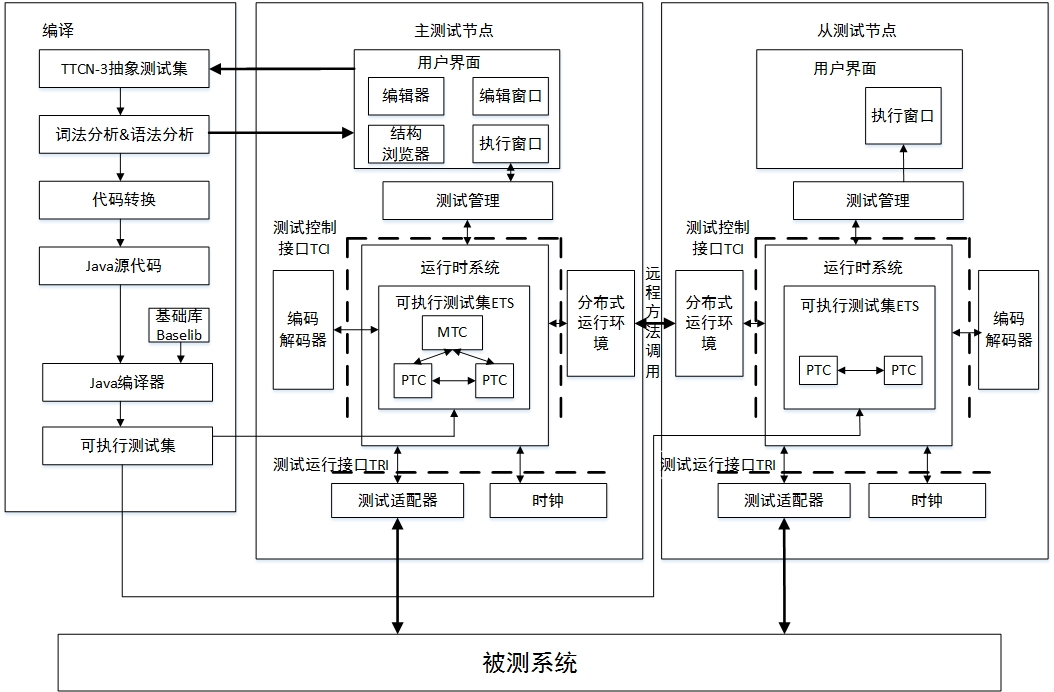
\includegraphics[width=0.75\textwidth]{pitsv3}
  \caption{PitSv3系统的体系结构\cite{journals_chinaf_YinWJS08}}
  \label{fig:pitsv3}
\end{figure}

\subsection{测试平台介绍}

\begin{figure}
  \centering
  % Requires \usepackage{graphicx}
  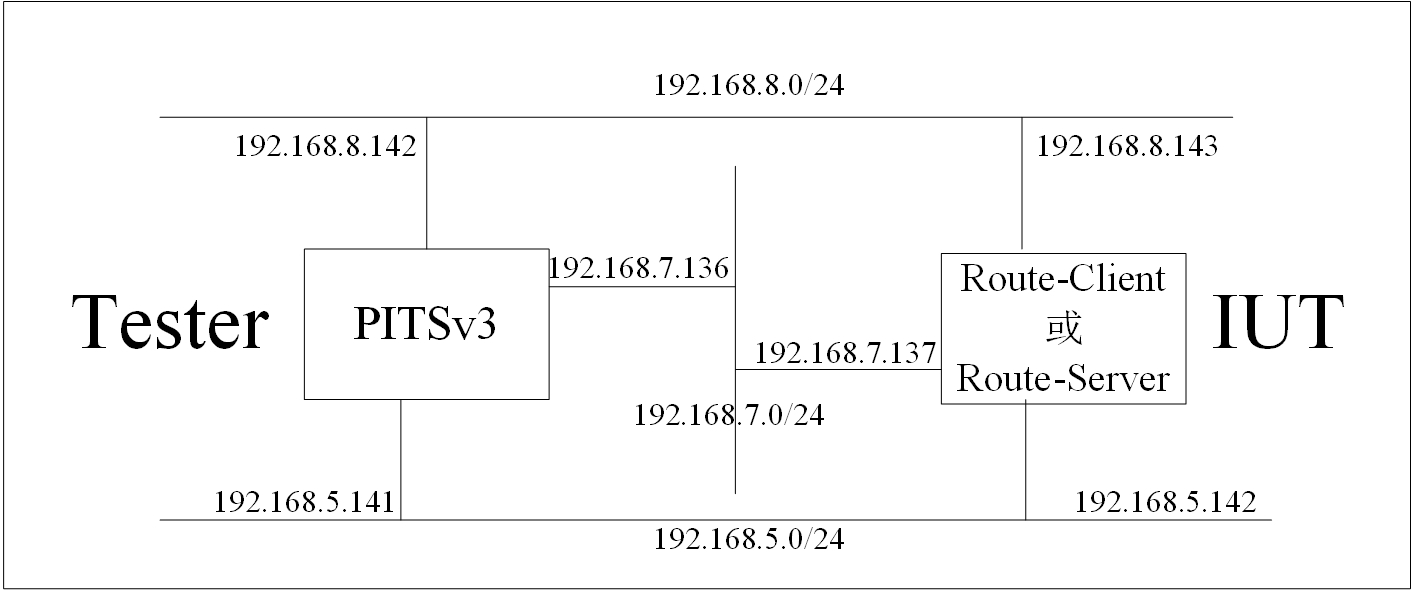
\includegraphics[width=0.8\textwidth]{environment}
  \caption{RSCP-iBGP系统的一致性测试环境}
  \label{fig:environment}
\end{figure}

\subsubsection{一致性测试工具及测试方法}
测试平台使用协议测试系统工具PITSv3\cite{journals_chinaf_YinWJS08}(Protocol Integrated Test System Version 3),PITSv3内通过主测试部件和多个从测试部件,来模拟测试系统多网口的情况,每个测试部件可以连接一个真实的虚拟路由器,以此来构建测试系统连接的网络拓扑,从而实现对协议的一致性测试。PITSv3系统的体系结构见图\ref{fig:pitsv3}。


协议测试系统工具PITSv3采用改进式的穿越测试法,测试系统和被测系统的多个接口分别相连接,测试系统通过和被测系统之间的报文交互,模拟被测系统外部真实的网络环境。如果被测设备周围连接了多个测试接口,则这多个测试接口对应为PITSv3软件中的一个主测试部件和多个从测试部件。


\subsubsection{一致性测试网络环境}
本文中针对RSCP-iBGP系统的功能测试,依托安装在物理机器上的VMware Workstation Pro虚拟机管理软件,在VMware虚拟机管理软件中运行多台虚拟机,分别作为测试系统和被测系统。虚拟机应设置内存(2G以上)、处理器个数(2个以上)、硬盘大小(20G以上)、网络适配器(通过VMware Workstation Pro虚拟机管理软件编辑栏下面的虚拟网络编辑器,添加网段进行网络配置)。

RSCP-iBGP系统的一致性测试主要测试部署RSCP-iBGP系统的自治系统内的Route-Server路由器和Route-Client路由器,该测试采用虚拟机的方式建立测试环境,该方式具有使用调试方便、部署迁移快速的优势。该测试启动两台虚拟机模拟网络环境。一台虚拟机作为测试系统,安装PITSv3的Windows系统。另一台虚拟机作为被测系统,运行RSCP-iBGP系统中的Route-Client软件路由器或者Route-Server软件路由器的Linux系统。具体的测试环境如图\ref{fig:environment}。

\subsection{一致性测试需求}

对RSCP-iBGP系统的测试主要分两个测试部分:对自治系统内的边界路由器Route-Client进行测试,对自治系统内的Route-Server进行测试,具体的测试需求如下。



% Please add the following required packages to your document preamble:
% \usepackage{booktabs}
\begin{table}[]
\centering
\caption{RSCP-iBGP系统中Route-Client与eBGP邻居的一致性测试集}
\label{tab:test1}
\begin{tabular}{@{}ccl@{}}
\toprule
测试组                                                                             & 测试用例     & 测试目的                                                                            \\ \midrule
\multirow{3}{*}{\begin{tabular}[c]{@{}c@{}}Route-Client与\\ eBGP邻居\end{tabular}} & 建连测试   & \begin{tabular}[c]{@{}l@{}}Route-Client可以接收\\ eBGP邻居的主动连接\end{tabular}        \\
                                                                                & 断连测试  & \begin{tabular}[c]{@{}l@{}}Route-Client可以处理\\ eBGP邻居的主动断连\end{tabular}        \\
                                                                                & 前缀报文接收测试 & \begin{tabular}[c]{@{}l@{}}Route-Client可以收到\\ eBGP邻居的UPDATE报文\end{tabular}   \\
                                                                                & 前缀报文处理测试 & \begin{tabular}[c]{@{}l@{}}Route-Client可将eBGP邻居\\ 的路由更新发给iBGP邻居\end{tabular} \\ \bottomrule
\end{tabular}
\end{table}

\subsubsection{被测系统Route-Client与eBGP邻居之间的测试}

被测系统Route-Client与eBGP邻居,进行eBGP邻居建连测试、eBGP邻居断连测试、eBGP邻居前缀报文接收测试、eBGP邻居前缀报文处理测试:

\paragraph{Route-Client与eBGP邻居建连测试}
测试系统软件向Route-Client被测系统发送OPEN报文,请求与Route-Client建立eBGP连接,当测试系统软件收到被测系统Route-Client回复过来的OPEN报文和KEEPALIVE报文,表明eBGP邻居建连成功;

\paragraph{Route-Client与eBGP邻居断连测试}
测试系统软件向Route-Client被测系统发送OPEN报文,请求与Route-Client建立eBGP连接,当测试系统软件收到被测系统Route-Client回复过来的OPEN报文和KEEPALIVE报文,则邻居建连成功,测试系统回复KEEPALIVE报文维持连接,之后测试系统主动断开BGP连接,即连续三次收到Route-Client被测系统发来的KEEPALIVE不回复,最后测试系统收到了Route-Client被测系统通知断连的NOTIFICATION报文,表明eBGP对等体断连成功;

\paragraph{Route-Client与eBGP邻居前缀报文接收测试}
测试系统软件和Route-Client被测系统建立eBGP连接,测试系统软件通过向Route-Client被测系统发送UPDATE报文信息,如果Route-Client被测系统正确接收到eBGP报文,Route-Client开启该eBGP对等体的Adj-RIB-In存储的情况下,能够查到收到的UPDATE报文信息,表明eBGP对等体前缀报文接收成功;

\paragraph{Route-Client与eBGP邻居前缀报文处理测试}
测试系统软件端口A和Route-Client被测系统建立eBGP连接,测试系统软件端口B和Route-Client被测系统建立iBGP连接。测试系统软件端口A通过向Route-Client被测系统发送UPDATE报文信息,如果Route-Client被测系统正确接收到eBGP报文,Route-Client开启该eBGP对等体的Adj-RIB-In存储的情况下,能够查到收到的UPDATE报文信息,表明eBGP对等体前缀报文接收成功;此时测试系统端口B收到了Route-Client发过来的携带Weight属性信息的UPDATE报文(配置Route-Client被测系统从某eBGP对等体收到路由的Weight值),表明eBGP对等体前缀报文处理正确。



\begin{table}[]
\centering
\caption{RSCP-iBGP系统中Route-Client与iBGP邻居的一致性测试集}
\label{tab:test2}
\begin{tabular}{@{}ccl@{}}
\toprule
测试组                                                                             & 测试用例     & \multicolumn{1}{c}{测试目的}                                                     \\ \midrule
\multirow{3}{*}{\begin{tabular}[c]{@{}c@{}}Route-Client与\\ iBGP邻居\end{tabular}} & 建连测试   & \begin{tabular}[c]{@{}l@{}}Route-Client可以接收\\ iBGP邻居的主动连接\end{tabular}       \\
                                                                                & 断连测试  & \begin{tabular}[c]{@{}l@{}}Route-Client可以处理\\ iBGP邻居的主动断连\end{tabular}       \\
                                                                                & 前缀报文接收测试 & \begin{tabular}[c]{@{}l@{}}Route-Client可以收到\\ iBGP邻居的UPDATE报文\end{tabular}  \\
                                                                                & 前缀报文处理测试 & \begin{tabular}[c]{@{}l@{}}Route-Client可将iBGP邻居\\ 的路由更新发给eBGP邻居\end{tabular} \\ \bottomrule
\end{tabular}
\end{table}

\subsubsection{被测系统Route-Client与iBGP邻居之间的测试}

被测系统Route-Client与iBGP邻居,进行iBGP邻居建连测试、iBGP邻居断连测试、iBGP邻居前缀报文接收测试、iBGP邻居前缀报文处理测试:

\paragraph{Route-Client与iBGP邻居建连测试}
测试系统软件向Route-Client被测系统发送OPEN报文,请求与Route-Client建立iBGP连接,当测试系统软件收到被测系统Route-Client回复过来的OPEN报文和KEEPALIVE报文,表明iBGP邻居建连成功;

\paragraph{Route-Client与iBGP邻居断连测试}
测试系统软件向Route-Client被测系统发送OPEN报文,请求与Route-Client建立iBGP连接,当测试系统软件收到被测系统Route-Client回复过来的OPEN报文和KEEPALIVE报文,则邻居建连成功,测试系统回复KEEPALIVE报文维持连接,之后测试系统主动断开BGP连接,即连续三次收到Route-Client被测系统发来的KEEPALIVE不回复,最后测试系统收到了Route-Client被测系统通知断连的NOTIFICATION报文,表明iBGP对等体断连成功;

\paragraph{Route-Client与iBGP邻居前缀报文接收测试}
测试系统软件和Route-Client被测系统建立iBGP连接,测试系统软件通过向Route-Client被测系统发送UPDATE报文信息,如果Route-Client被测系统正确接收到iBGP报文,Route-Client开启该iBGP对等体的Adj-RIB-In存储的情况下,能够查到收到的UPDATE报文信息,表明iBGP对等体前缀报文接收成功;

\paragraph{Route-Client与iBGP邻居前缀报文处理测试}
测试系统软件端口A和Route-Client被测系统建立eBGP连接,测试系统软件端口B和Route-Client被测系统建立eBGP连接,测试系统软件端口C和Route-Client被测系统建立iBGP连接。测试系统软件端口C通过向Route-Client被测系统发送UPDATE报文信息,如果Route-Client被测系统正确接收到iBGP报文,Route-Client开启该iBGP对等体的Adj-RIB-In存储的情况下,能够查到收到的UPDATE报文信息,表明iBGP对等体前缀报文接收成功;此时测试系统端口A和B收到了Route-Client转发过来的从iBGP收到的前缀的最优路由的UPDATE报文,表明iBGP对等体前缀报文处理正确。






\begin{table}[]
\centering
\caption{RSCP-iBGP系统中Route-Server与iBGP邻居的一致性测试集}
\label{tab:test3}
\begin{tabular}{@{}ccl@{}}
\toprule
测试组                                                                             & 测试用例     & \multicolumn{1}{c}{测试目的}                                                                        \\ \midrule
\multirow{3}{*}{\begin{tabular}[c]{@{}c@{}}Route-Server与\\ iBGP邻居\end{tabular}} & 建连测试     & \begin{tabular}[c]{@{}l@{}}Route-Server可以接收\\ iBGP邻居的主动连接\end{tabular}                          \\
                                                                                & 断连测试     & \begin{tabular}[c]{@{}l@{}}Route-Server可以处理\\ iBGP邻居的主动断连\end{tabular}                          \\
                                                                                & 前缀报文接收测试 & \begin{tabular}[c]{@{}l@{}}Route-Server可以收到iBGP邻居\\ 的带有Weight属性值的UPDATE报文\end{tabular}          \\
                                                                                & 前缀报文处理测试 & \begin{tabular}[c]{@{}l@{}}Route-Server收到iBGP邻居的路由更新,计算\\ iBGP邻居对应最优路由并宣告给每个iBGP邻居\end{tabular} \\ \bottomrule
\end{tabular}
\end{table}

\subsubsection{被测系统Route-Server与iBGP邻居之间的测试}

被测系统Route-Server与iBGP邻居,进行iBGP邻居建连测试、iBGP邻居断连测试、iBGP邻居前缀报文接收测试、iBGP邻居前缀报文处理测试:

\paragraph{Route-Server与iBGP邻居建连测试}
测试系统软件向Route-Server被测系统发送OPEN报文,请求与Route-Server建立iBGP连接,当测试系统软件收到被测系统Route-Server回复过来的OPEN报文和KEEPALIVE报文,表明iBGP邻居建连成功;

\paragraph{Route-Server与iBGP邻居断连测试}
被测系统Route-Server与iBGP邻居,进行iBGP对等体断连测试:测试系统软件向Route-Server被测系统发送OPEN报文,请求与Route-Server建立iBGP连接,当测试系统软件收到被测系统Route-Server回复过来的OPEN报文和KEEPALIVE报文,则邻居建连成功,测试系统回复KEEPALIVE报文维持连接,之后测试系统主动断开BGP连接,即连续三次收到Route-Server被测系统发来的KEEPALIVE不回复,最后测试系统收到了Route-Server被测系统通知断连的NOTIFICATION报文,表明iBGP对等体断连成功;

\paragraph{Route-Server与iBGP邻居前缀报文接收测试}
测试系统软件和Route-Server被测系统建立iBGP连接,测试系统软件通过向Route-Server被测系统发送UPDATE报文信息,如果Route-Server被测系统正确接收到携带Weight属性信息的UPDATE报文,表明iBGP对等体前缀报文接收成功;

\begin{figure}
  \centering
  % Requires \usepackage{graphicx}
  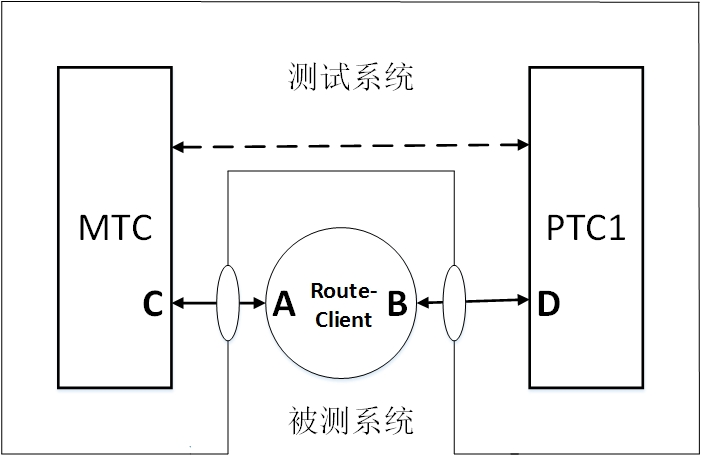
\includegraphics[width=0.6\textwidth]{conf}
  \caption{Route-Client与eBGP邻居前缀报文处理的测试配置}
  \label{fig:conf}
\end{figure}

\paragraph{Route-Server与iBGP邻居前缀报文处理测试}
测试系统软件端口A和Route-Server被测系统建立iBGP连接,测试系统软件端口B和Route-Server被测系统建立iBGP连接,测试系统软件端口C和Route-Server被测系统建立iBGP连接。测试系统软件端口A通过向Route-Server被测系统发送2条相同前缀不同路由的UPDATE报文信息,如果Route-Server被测系统正确接收到该2条路由信息,表明iBGP对等体前缀报文接收成功;此时测试系统端口A、B和C收到了Route-Server被测系统发来的该前缀的最优路由的UPDATE报文,表明被测系统Route-Server与iBGP对等体之间的前缀报文处理正确。




\subsection{测试集设计}

\begin{figure}
  \centering
  % Requires \usepackage{graphicx}
  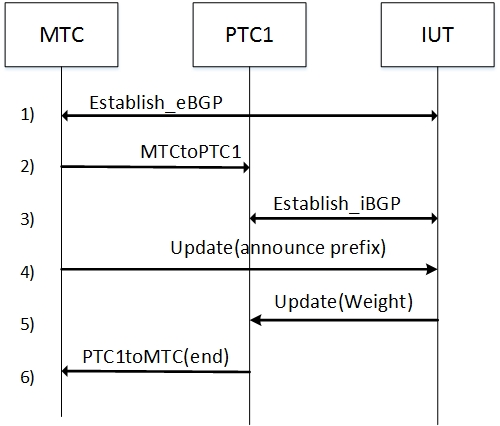
\includegraphics[width=0.6\textwidth]{seq}
  \caption{Route-Client与eBGP邻居前缀报文处理的测试序列}
  \label{fig:seq}
\end{figure}

本文提出的RSCP-iBGP系统在自治系统内部有两种类型的路由器:边界路由器Route-Client和集中平台上的Route-Server,Route-Client路由器有eBGP对等体和iBGP对等体,而Route-Server路由器仅有iBGP对等体。根据测试需求设计三组测试集共3组:Route-Client与eBGP邻居之间的一致性测试集如表\ref{tab:test1}、Route-Client与iBGP邻居之间的一致性测试集如表\ref{tab:test2}、Route-Server与iBGP邻居之间的一致性测试集如表\ref{tab:test3}。

被测系统和测试系统之间通过报文交互完成测试过程,以Route-Client与eBGP邻居前缀报文处理测试为例,其测试配置如图\ref{fig:conf}。在该测试例中模拟被测系统Route-Client有2个邻居,在测试系统中使用一个主测试部件MTC模拟被测系统的eBGP邻居C,使用一个从测试部件PTC1模拟被测系统的iBGP邻居D。

在RSCP-iBGP系统中,Route-Client收到eBGP路由经过入站过滤后,会将携带Weight路径属性值的路由发到集中平台。则C口与Route-Client建立eBGP连接,C口向Route-Client宣告路由,Route-Client会将经过入站策略的该路由信息携带Weight属性值发给iBGP邻居(D口)。



Route-Client与eBGP邻居前缀报文处理的测试序列见图\ref{fig:seq},其测试序列对应的流程描述如下:

\begin{enumerate}[1)]
  \item MTC模拟对等体C主动与被测系统A口建立eBGP连接;
  \item MTC通知PTC1:对等体C已经和被测系统A口建立连接。对等体D可以与被测系统的B口建立iBGP连接;
  \item PTC1模拟对等体D与被测系统的B口建立iBGP连接;
  \item 测试系统从C口向被测系统的A口宣告路由192.168.1.0/24;
  \item 测试系统从D口收到携带Weight值且Next-hop地址为C口地址的192.168.1.0/24的路由信息;
  \item PTC1通知MTC:测试系统D口收到了正确UPDATE报文,测试结束。
\end{enumerate}

如果Route-Client与eBGP邻居前缀报文处理的测试例在运行的过程中遵循图\ref{fig:seq}的测试序列,则测试例PASS,否则测试例FAIL。



\subsection{测试结果及分析}


\begin{figure}
  \centering
  % Requires \usepackage{graphicx}
  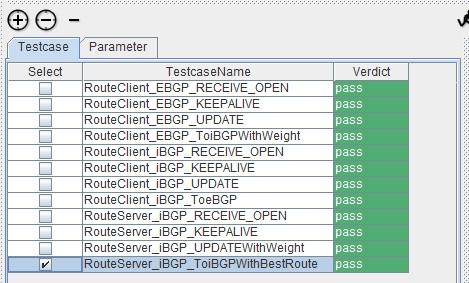
\includegraphics[width=0.8\textwidth]{test}
  \caption{RSCP-iBGP系统测试集的测试界面}
  \label{fig:test}
\end{figure}


针对以上的测试需求和测试方案,本文对3组测试集进行了测试,测试例全部通过,PITSv3软件的测试界面如图\ref{fig:test}。

表\ref{tab:res}所示是RSCP-iBGP系统的测试结果统计,从表中我们可以看出测试例全部通过。RSCP-iBGP系统中的Route-Client路由器和Route-Server可以进行正常的BGP协议下的报文交互,Route-Client路由器收到eBGP路由,会将其经过入站策略且携带Weight属性的路由信息传输到集中平台上的Route-Server路由器,Route-Server会计算出每台边界路由器针对该Prefix的最优路由,并将其传输给域内的每一台边界路由器Route-Client,之后Route-Client将收到的iBGP路由宣告给所有的eBGP邻居,整个路由处理的流程在RSCP-iBGP系统中均正确无误,证明RSCP-iBGP系统实现与设计规范的一致性。


% Please add the following required packages to your document preamble:
% \usepackage{booktabs}
\begin{table}[]
\centering
\caption{RSCP-iBGP系统一致性测试集的测试结果}
\label{tab:res}
\begin{tabular}{@{}ccc@{}}
\toprule
测试集名称               & 通过用例数 & 失败用例数 \\ \midrule
Route-Client与eBGP邻居 & 4     & 0     \\
Route-Client与iBGP邻居 & 4     & 0     \\
Route-Server与iBGP邻居 & 4     & 0     \\
总计                  & 12    & 0     \\ \bottomrule
\end{tabular}
\end{table}


\section{本章小结}

本章主要对RSCP-iBGP系统的进行了功能验证、BGP扩展协议一致性测试。通过本章的仿真实验和协议测试,本文实现的RSCP-iBGP系统在功能实现上达到了最初的设计目标:基于全部路由进行路由计算,集合缩小式的新型路由算法也能避免MED不可比引起的路由震荡,路由表在集中平台上存储优化。在本文提出的RSCP-iBGP系统中,自治系统内部的路由计算次数和路由存储大小均优化了一个数量级,且不存在路由震荡和路由收敛等情况。

\chapter{总结与展望}
\label{cha:china}



\section{主要结论}
结论、创新点


\section{未来工作}
集中配置策略、优化ebgp邻居连接

%%% 其它部分
\backmatter

%% 本科生要这几个索引,研究生不要。选择性留下。
% 插图索引
%\listoffigures
% 表格索引
%\listoftables
% 公式索引
%\listofequations


%% 参考文献
% 注意:至少需要引用一篇参考文献,否则下面两行可能引起编译错误。
% 如果不需要参考文献,请将下面两行删除或注释掉。
% 数字式引用

\bibliographystyle{thuthesis-numeric}
% 作者-年份式引用
%\bibliographystyle{thuthesis-author-year}
%\bibliographystyle{thubib}
\bibliography{ref/refs}


%% 致谢
% 如果使用声明扫描页,将可选参数指定为扫描后的 PDF 文件名,例如:
% \begin{acknowledgement}[scan-statement.pdf]
\begin{acknowledgement}
  衷心感谢导师尹霞教授,在我读硕士期间对我的关心和指导,并言传身教引导我树立严谨的科研态度和认真踏实的做事原则。在我科研长时间停滞不前的阶段,是尹霞老师的鼓励和支持,帮助我重拾科研的信心,语重心长地告诫我在科研上投入的时间不足,应“先做减法,再做加法”,让我迅速走出了科研困境。尹霞老师对实验室的同学都非常爱护,切身考虑同学们的处境和需要,关键时刻给我们很多精神上的大力支持和切合实际的宝贵建议,特别是在我毕业找工作的过程中,给予了我很多的帮助和建议。她不仅是我科研上的引领者,更是我人生的导师。

  万分感谢我的辅导老师王之梁老师,他批判性的科研思维和细致严谨的科研习惯,时时刻刻影响着我。硕士期间王老师一直悉心指导我的科研,定期与我讨论,明确指出我在科研上的一些陋习和思维缺陷,帮助我在科研上不断成长和进步。王老师在科研上对我的指导非常细致,有时我在实验阶段遇到瓶颈,王老师会亲自帮我查看并调试,我也能从中学习老师解决实际问题的方法,非常感激老师。以后在学习新东西的过程中,我也将继续保持在王老师教诲下养成的良好思维习惯及学习方式。

  非常感谢施新刚老师、姚姜源老师,他们对我在实验室的学习给了很大的帮助和支持。

  感谢实验室余家傲老师、张娜老师对我生活上的帮助,为实验室的同学创造了良好的科研环境。感谢实验室的张晗、郭迎亚、赵宗义、李亚慧、杨言、王苏、刘智峰、陈志鹏、马强、田莹等同学的帮助和鼓励,和他们的讨论帮助我解决了很多科研上的盲点,他们对我的鼓励促使我更加用心地投入到科研,感谢你们!


  %感谢 \LaTeX 和 \thuthesis\cite{thuthesis},帮我节省了不少时间。
\end{acknowledgement}


%% 附录
%\begin{appendix}
%\chapter{外文资料原文}
\label{cha:engorg}

\title{The title of the English paper}

\textbf{Abstract:} As one of the most widely used techniques in operations
research, \emph{ mathematical programming} is defined as a means of maximizing a
quantity known as \emph{bjective function}, subject to a set of constraints
represented by equations and inequalities. Some known subtopics of mathematical
programming are linear programming, nonlinear programming, multiobjective
programming, goal programming, dynamic programming, and multilevel
programming$^{[1]}$.

It is impossible to cover in a single chapter every concept of mathematical
programming. This chapter introduces only the basic concepts and techniques of
mathematical programming such that readers gain an understanding of them
throughout the book$^{[2,3]}$.


\section{Single-Objective Programming}
The general form of single-objective programming (SOP) is written
as follows,
\begin{equation}\tag*{(123)} % 如果附录中的公式不想让它出现在公式索引中,那就请
                             % 用 \tag*{xxxx}
\left\{\begin{array}{l}
\max \,\,f(x)\\[0.1 cm]
\mbox{subject to:} \\ [0.1 cm]
\qquad g_j(x)\le 0,\quad j=1,2,\cdots,p
\end{array}\right.
\end{equation}
which maximizes a real-valued function $f$ of
$x=(x_1,x_2,\cdots,x_n)$ subject to a set of constraints.

\newtheorem{mpdef}{Definition}[chapter]
\begin{mpdef}
In SOP, we call $x$ a decision vector, and
$x_1,x_2,\cdots,x_n$ decision variables. The function
$f$ is called the objective function. The set
\begin{equation}\tag*{(456)} % 这里同理,其它不再一一指定。
S=\left\{x\in\Re^n\bigm|g_j(x)\le 0,\,j=1,2,\cdots,p\right\}
\end{equation}
is called the feasible set. An element $x$ in $S$ is called a
feasible solution.
\end{mpdef}

\newtheorem{mpdefop}[mpdef]{Definition}
\begin{mpdefop}
A feasible solution $x^*$ is called the optimal
solution of SOP if and only if
\begin{equation}
f(x^*)\ge f(x)
\end{equation}
for any feasible solution $x$.
\end{mpdefop}

One of the outstanding contributions to mathematical programming was known as
the Kuhn-Tucker conditions\ref{eq:ktc}. In order to introduce them, let us give
some definitions. An inequality constraint $g_j(x)\le 0$ is said to be active at
a point $x^*$ if $g_j(x^*)=0$. A point $x^*$ satisfying $g_j(x^*)\le 0$ is said
to be regular if the gradient vectors $\nabla g_j(x)$ of all active constraints
are linearly independent.

Let $x^*$ be a regular point of the constraints of SOP and assume that all the
functions $f(x)$ and $g_j(x),j=1,2,\cdots,p$ are differentiable. If $x^*$ is a
local optimal solution, then there exist Lagrange multipliers
$\lambda_j,j=1,2,\cdots,p$ such that the following Kuhn-Tucker conditions hold,
\begin{equation}
\label{eq:ktc}
\left\{\begin{array}{l}
    \nabla f(x^*)-\sum\limits_{j=1}^p\lambda_j\nabla g_j(x^*)=0\\[0.3cm]
    \lambda_jg_j(x^*)=0,\quad j=1,2,\cdots,p\\[0.2cm]
    \lambda_j\ge 0,\quad j=1,2,\cdots,p.
\end{array}\right.
\end{equation}
If all the functions $f(x)$ and $g_j(x),j=1,2,\cdots,p$ are convex and
differentiable, and the point $x^*$ satisfies the Kuhn-Tucker conditions
(\ref{eq:ktc}), then it has been proved that the point $x^*$ is a global optimal
solution of SOP.

\subsection{Linear Programming}
\label{sec:lp}

If the functions $f(x),g_j(x),j=1,2,\cdots,p$ are all linear, then SOP is called
a {\em linear programming}.

The feasible set of linear is always convex. A point $x$ is called an extreme
point of convex set $S$ if $x\in S$ and $x$ cannot be expressed as a convex
combination of two points in $S$. It has been shown that the optimal solution to
linear programming corresponds to an extreme point of its feasible set provided
that the feasible set $S$ is bounded. This fact is the basis of the {\em simplex
  algorithm} which was developed by Dantzig as a very efficient method for
solving linear programming.
\begin{table}[ht]
\centering
  \centering
  \caption*{Table~1\hskip1em This is an example for manually numbered table, which
    would not appear in the list of tables}
  \label{tab:badtabular2}
  \begin{tabular}[c]{|m{1.5cm}|c|c|c|c|c|c|}\hline
    \multicolumn{2}{|c|}{Network Topology} & \# of nodes &
    \multicolumn{3}{c|}{\# of clients} & Server \\\hline
    GT-ITM & Waxman Transit-Stub & 600 &
    \multirow{2}{2em}{2\%}&
    \multirow{2}{2em}{10\%}&
    \multirow{2}{2em}{50\%}&
    \multirow{2}{1.2in}{Max. Connectivity}\\\cline{1-3}
    \multicolumn{2}{|c|}{Inet-2.1} & 6000 & & & &\\\hline
    \multirow{2}{1.5cm}{Xue} & Rui  & Ni &\multicolumn{4}{c|}{\multirow{2}*{\thuthesis}}\\\cline{2-3}
    & \multicolumn{2}{c|}{ABCDEF} &\multicolumn{4}{c|}{} \\\hline
\end{tabular}
\end{table}

Roughly speaking, the simplex algorithm examines only the extreme points of the
feasible set, rather than all feasible points. At first, the simplex algorithm
selects an extreme point as the initial point. The successive extreme point is
selected so as to improve the objective function value. The procedure is
repeated until no improvement in objective function value can be made. The last
extreme point is the optimal solution.

\subsection{Nonlinear Programming}

If at least one of the functions $f(x),g_j(x),j=1,2,\cdots,p$ is nonlinear, then
SOP is called a {\em nonlinear programming}.

A large number of classical optimization methods have been developed to treat
special-structural nonlinear programming based on the mathematical theory
concerned with analyzing the structure of problems.
\begin{figure}[h]
  \centering
  
\includegraphics{thu-lib-logo}
  \caption*{Figure~1\quad This is an example for manually numbered figure,
    which would not appear in the list of figures}
  \label{tab:badfigure2}
\end{figure}

Now we consider a nonlinear programming which is confronted solely with
maximizing a real-valued function with domain $\Re^n$.  Whether derivatives are
available or not, the usual strategy is first to select a point in $\Re^n$ which
is thought to be the most likely place where the maximum exists. If there is no
information available on which to base such a selection, a point is chosen at
random. From this first point an attempt is made to construct a sequence of
points, each of which yields an improved objective function value over its
predecessor. The next point to be added to the sequence is chosen by analyzing
the behavior of the function at the previous points. This construction continues
until some termination criterion is met. Methods based upon this strategy are
called {\em ascent methods}, which can be classified as {\em direct methods},
{\em gradient methods}, and {\em Hessian methods} according to the information
about the behavior of objective function $f$. Direct methods require only that
the function can be evaluated at each point. Gradient methods require the
evaluation of first derivatives of $f$. Hessian methods require the evaluation
of second derivatives. In fact, there is no superior method for all
problems. The efficiency of a method is very much dependent upon the objective
function.

\subsection{Integer Programming}

{\em Integer programming} is a special mathematical programming in which all of
the variables are assumed to be only integer values. When there are not only
integer variables but also conventional continuous variables, we call it {\em
  mixed integer programming}. If all the variables are assumed either 0 or 1,
then the problem is termed a {\em zero-one programming}. Although integer
programming can be solved by an {\em exhaustive enumeration} theoretically, it
is impractical to solve realistically sized integer programming problems. The
most successful algorithm so far found to solve integer programming is called
the {\em branch-and-bound enumeration} developed by Balas (1965) and Dakin
(1965). The other technique to integer programming is the {\em cutting plane
  method} developed by Gomory (1959).

\hfill\textit{Uncertain Programming\/}\quad(\textsl{BaoDing Liu, 2006.2})

\section*{References}
\noindent{\itshape NOTE: These references are only for demonstration. They are
  not real citations in the original text.}

\begin{translationbib}
\item Donald E. Knuth. The \TeX book. Addison-Wesley, 1984. ISBN: 0-201-13448-9
\item Paul W. Abrahams, Karl Berry and Kathryn A. Hargreaves. \TeX\ for the
  Impatient. Addison-Wesley, 1990. ISBN: 0-201-51375-7
\item David Salomon. The advanced \TeX book.  New York : Springer, 1995. ISBN:0-387-94556-3
\end{translationbib}

\chapter{外文资料的调研阅读报告或书面翻译}

\title{英文资料的中文标题}

{\heiti 摘要:} 本章为外文资料翻译内容。如果有摘要可以直接写上来,这部分好像没有
明确的规定。

\section{单目标规划}
北冥有鱼,其名为鲲。鲲之大,不知其几千里也。化而为鸟,其名为鹏。鹏之背,不知其几
千里也。怒而飞,其翼若垂天之云。是鸟也,海运则将徙于南冥。南冥者,天池也。
\begin{equation}\tag*{(123)}
 p(y|\mathbf{x}) = \frac{p(\mathbf{x},y)}{p(\mathbf{x})}=
\frac{p(\mathbf{x}|y)p(y)}{p(\mathbf{x})}
\end{equation}

吾生也有涯,而知也无涯。以有涯随无涯,殆已!已而为知者,殆而已矣!为善无近名,为
恶无近刑,缘督以为经,可以保身,可以全生,可以养亲,可以尽年。

\subsection{线性规划}
庖丁为文惠君解牛,手之所触,肩之所倚,足之所履,膝之所倚,砉然响然,奏刀騞然,莫
不中音,合于桑林之舞,乃中经首之会。
\begin{table}[ht]
\centering
  \centering
  \caption*{表~1\hskip1em 这是手动编号但不出现在索引中的一个表格例子}
  \label{tab:badtabular3}
  \begin{tabular}[c]{|m{1.5cm}|c|c|c|c|c|c|}\hline
    \multicolumn{2}{|c|}{Network Topology} & \# of nodes &
    \multicolumn{3}{c|}{\# of clients} & Server \\\hline
    GT-ITM & Waxman Transit-Stub & 600 &
    \multirow{2}{2em}{2\%}&
    \multirow{2}{2em}{10\%}&
    \multirow{2}{2em}{50\%}&
    \multirow{2}{1.2in}{Max. Connectivity}\\\cline{1-3}
    \multicolumn{2}{|c|}{Inet-2.1} & 6000 & & & &\\\hline
    \multirow{2}{1.5cm}{Xue} & Rui  & Ni &\multicolumn{4}{c|}{\multirow{2}*{\thuthesis}}\\\cline{2-3}
    & \multicolumn{2}{c|}{ABCDEF} &\multicolumn{4}{c|}{} \\\hline
\end{tabular}
\end{table}

文惠君曰:“嘻,善哉!技盖至此乎?”庖丁释刀对曰:“臣之所好者道也,进乎技矣。始臣之
解牛之时,所见无非全牛者;三年之后,未尝见全牛也;方今之时,臣以神遇而不以目视,
官知止而神欲行。依乎天理,批大郤,导大窾,因其固然。技经肯綮之未尝,而况大坬乎!
良庖岁更刀,割也;族庖月更刀,折也;今臣之刀十九年矣,所解数千牛矣,而刀刃若新发
于硎。彼节者有间而刀刃者无厚,以无厚入有间,恢恢乎其于游刃必有余地矣。是以十九年
而刀刃若新发于硎。虽然,每至于族,吾见其难为,怵然为戒,视为止,行为迟,动刀甚微,
謋然已解,如土委地。提刀而立,为之而四顾,为之踌躇满志,善刀而藏之。”

文惠君曰:“善哉!吾闻庖丁之言,得养生焉。”


\subsection{非线性规划}
孔子与柳下季为友,柳下季之弟名曰盗跖。盗跖从卒九千人,横行天下,侵暴诸侯。穴室枢
户,驱人牛马,取人妇女。贪得忘亲,不顾父母兄弟,不祭先祖。所过之邑,大国守城,小
国入保,万民苦之。孔子谓柳下季曰:“夫为人父者,必能诏其子;为人兄者,必能教其弟。
若父不能诏其子,兄不能教其弟,则无贵父子兄弟之亲矣。今先生,世之才士也,弟为盗
跖,为天下害,而弗能教也,丘窃为先生羞之。丘请为先生往说之。”
\begin{figure}[h]
  \centering
  
\includegraphics{thu-whole-logo}
  \caption*{图~1\hskip1em 这是手动编号但不出现索引中的图片的例子}
  \label{tab:badfigure3}
\end{figure}

柳下季曰:“先生言为人父者必能诏其子,为人兄者必能教其弟,若子不听父之诏,弟不受
兄之教,虽今先生之辩,将奈之何哉?且跖之为人也,心如涌泉,意如飘风,强足以距敌,
辩足以饰非。顺其心则喜,逆其心则怒,易辱人以言。先生必无往。”

孔子不听,颜回为驭,子贡为右,往见盗跖。

\subsection{整数规划}
盗跖乃方休卒徒大山之阳,脍人肝而餔之。孔子下车而前,见谒者曰:“鲁人孔丘,闻将军
高义,敬再拜谒者。”谒者入通。盗跖闻之大怒,目如明星,发上指冠,曰:“此夫鲁国之
巧伪人孔丘非邪?为我告之:尔作言造语,妄称文、武,冠枝木之冠,带死牛之胁,多辞缪
说,不耕而食,不织而衣,摇唇鼓舌,擅生是非,以迷天下之主,使天下学士不反其本,妄
作孝弟,而侥幸于封侯富贵者也。子之罪大极重,疾走归!不然,我将以子肝益昼餔之膳。”


\chapter{其它附录}
前面两个附录主要是给本科生做例子。其它附录的内容可以放到这里,当然如果你愿意,可
以把这部分也放到独立的文件中,然后将其 \cs{input} 到主文件中。

%\end{appendix}

%% 个人简历
\begin{resume}

  \resumeitem{个人简历}

  xxxx 年 xx 月 xx 日出生于 xx 省 xx 县。

  xxxx 年 9 月考入 xx 大学 xx 系 xx 专业,xxxx 年 7 月本科毕业并获得 xx 学士学位。

  xxxx 年 9 月免试进入 xx 大学 xx 系攻读 xx 学位至今。

  \researchitem{发表的学术论文} % 发表的和录用的合在一起

  % 1. 已经刊载的学术论文(本人是第一作者,或者导师为第一作者本人是第二作者)
  \begin{publications}
    \item Yang Y, Ren T L, Zhang L T, et al. Miniature microphone with silicon-
      based ferroelectric thin films. Integrated Ferroelectrics, 2003,
      52:229-235. (SCI 收录, 检索号:758FZ.)
    \item 杨轶, 张宁欣, 任天令, 等. 硅基铁电微声学器件中薄膜残余应力的研究. 中国机
      械工程, 2005, 16(14):1289-1291. (EI 收录, 检索号:0534931 2907.)
    \item 杨轶, 张宁欣, 任天令, 等. 集成铁电器件中的关键工艺研究. 仪器仪表学报,
      2003, 24(S4):192-193. (EI 源刊.)
  \end{publications}

  % 2. 尚未刊载,但已经接到正式录用函的学术论文(本人为第一作者,或者
  %    导师为第一作者本人是第二作者)。
  \begin{publications}[before=\publicationskip,after=\publicationskip]
    \item Yang Y, Ren T L, Zhu Y P, et al. PMUTs for handwriting recognition. In
      press. (已被 Integrated Ferroelectrics 录用. SCI 源刊.)
  \end{publications}

  % 3. 其他学术论文。可列出除上述两种情况以外的其他学术论文,但必须是
  %    已经刊载或者收到正式录用函的论文。
  \begin{publications}
    \item Wu X M, Yang Y, Cai J, et al. Measurements of ferroelectric MEMS
      microphones. Integrated Ferroelectrics, 2005, 69:417-429. (SCI 收录, 检索号
      :896KM)
    \item 贾泽, 杨轶, 陈兢, 等. 用于压电和电容微麦克风的体硅腐蚀相关研究. 压电与声
      光, 2006, 28(1):117-119. (EI 收录, 检索号:06129773469)
    \item 伍晓明, 杨轶, 张宁欣, 等. 基于MEMS技术的集成铁电硅微麦克风. 中国集成电路,
      2003, 53:59-61.
  \end{publications}

  \researchitem{研究成果} % 有就写,没有就删除
  \begin{achievements}
    \item 任天令, 杨轶, 朱一平, 等. 硅基铁电微声学传感器畴极化区域控制和电极连接的
      方法: 中国, CN1602118A. (中国专利公开号)
    \item Ren T L, Yang Y, Zhu Y P, et al. Piezoelectric micro acoustic sensor
      based on ferroelectric materials: USA, No.11/215, 102. (美国发明专利申请号)
  \end{achievements}

\end{resume}


%% 本科生进行格式审查是需要下面这个表格,答辩可能不需要。选择性留下。
% 综合论文训练记录表
%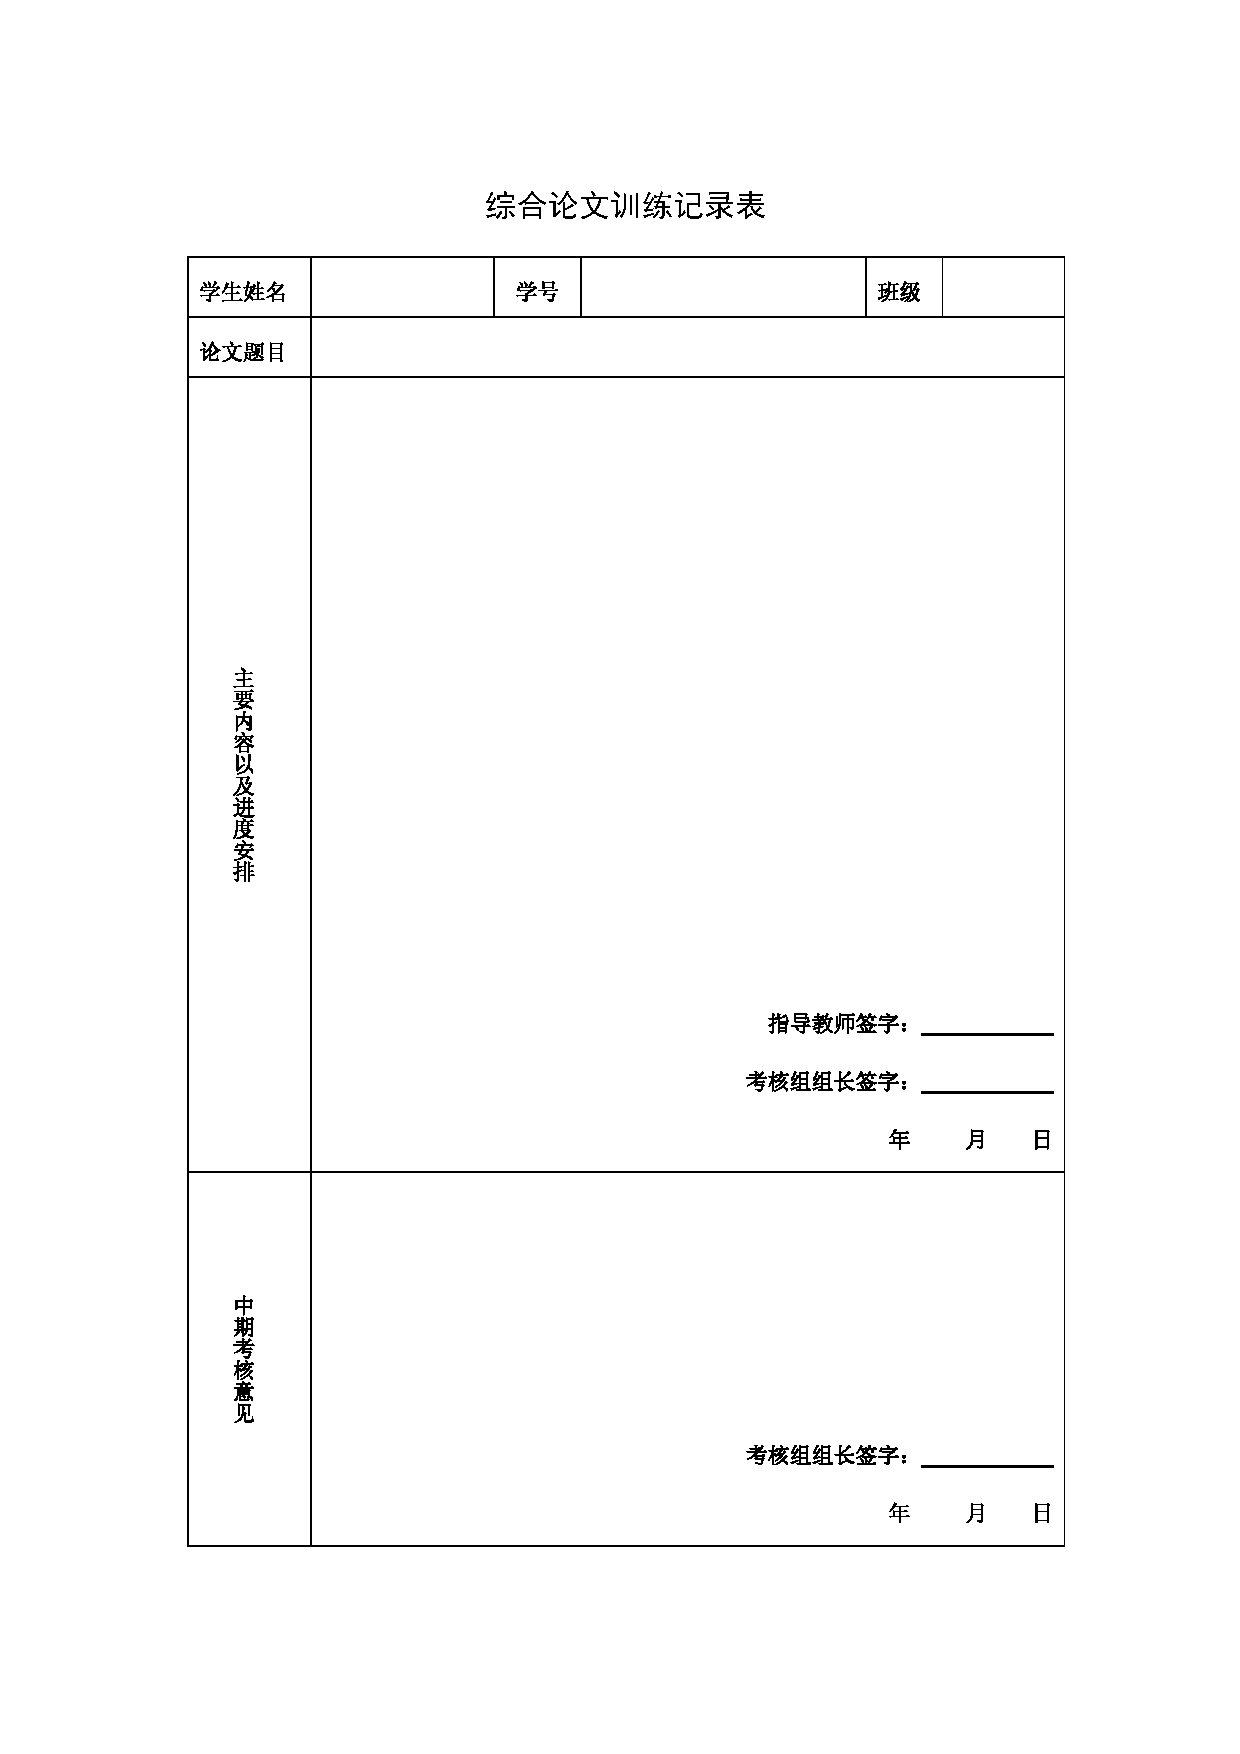
\includepdf[pages=-]{scan-record.pdf}
\end{document}
